%For final camera-ready submission, w/ required CCS and ACM Reference
% \documentclass[acmsmall]{acmart}\settopmatter{}
\documentclass[acmsmall,screen]{acmart} 
% Anshuman is maintaining an issue list at
% https://docs.google.com/spreadsheets/d/11_lN7I7RnIjRcRAW_zyK4x03sH7-aA9oEyiyhlPlxP0/edit?usp=sharing

%% Conference information
%% Supplied to authors by publisher for camera-ready submission;
%% use defaults for review submission.
%% \acmConference[OOPSLA '19]{Proceedings of the ACM on Programming Languages, Volume 3, Number OOPSLA}{October 20–25, 2019}{Athens, Greece}
%% \acmISBN{} % \acmISBN{978-x-xxxx-xxxx-x/YY/MM}
\startPage{1}

%% Copyright information
%% Supplied to authors (based on authors' rights management selection;
%% see authors.acm.org) by publisher for camera-ready submission;
%% use 'none' for review submission.
% \setcopyright{none}
%% \setcopyright{acmcopyright}
%\setcopyright{acmlicensed}
\setcopyright{rightsretained}
\acmPrice{}
\acmDOI{10.1145/3360597}
\acmYear{2019}
\copyrightyear{2019}
\acmJournal{PACMPL}
\acmVolume{3}
\acmNumber{OOPSLA}
\acmArticle{171}
\acmMonth{10}

%% Bibliography style
\bibliographystyle{ACM-Reference-Format}
%% Citation style
\citestyle{acmauthoryear}  %% For author/year citations
%\citestyle{acmnumeric}     %% For numeric citations
%\setcitestyle{nosort}      %% With 'acmnumeric', to disable automatic
                            %% sorting of references within a single citation;
                            %% e.g., \cite{Smith99,Carpenter05,Baker12}
                            %% rendered as [14,5,2] rather than [2,5,14].
%\setcitesyle{nocompress}   %% With 'acmnumeric', to disable automatic
                            %% compression of sequential references within a
                            %% single citation;
                            %% e.g., \cite{Baker12,Baker14,Baker16}
                            %% rendered as [2,3,4] rather than [2-4].


%%%%%%%%%%%%%%%%%%%%%%%%%%%%%%%%%%%%%%%%%%%%%%%%%%%%%%%%%%%%%%%%%%%%%%
%% Note: Authors migrating a paper from traditional SIGPLAN
%% proceedings format to PACMPL format must update the
%% '\documentclass' and topmatter commands above; see
%% 'acmart-pacmpl-template.tex'.
%%%%%%%%%%%%%%%%%%%%%%%%%%%%%%%%%%%%%%%%%%%%%%%%%%%%%%%%%%%%%%%%%%%%%%

%% Some recommended packages.
%\usepackage{booktabs}   %% For formal tables:
                        %% http://ctan.org/pkg/booktabs
%\usepackage{subcaption} %% For complex figures with subfigures/subcaptions
                        %% http://ctan.org/pkg/subcaption

\usepackage{listings}          % for code formatting
\usepackage{stmaryrd}          % for the lightning symbol
\usepackage{mathtools}         % for mathrlap
\usepackage{semantic}          % for mathlig
\usepackage{mathpartir}        % for inferrule
\usepackage{tikz}              % for drawings
\usepackage{courier}           % for the courier font (optional)
\usepackage{multicol}          % for multi-column listings
\usepackage{subcaption}        % for subfigures
\usepackage[export]{adjustbox} % for subfigures
\usepackage{accents}
\usepackage{wrapfig}
\usepackage{scalerel}
\usepackage{graphicx}
\usepackage{fvextra}

\renewcommand*{\ttdefault}{zi4}

% inline code
\makeatletter
\newlength{\@mli}
\newcommand{\mli}[1]{%
  \settowidth{\@mli}{\lstinline/#1/}
  \hspace{-.5ex}\begin{minipage}[t]{\@mli}\lstinline/#1/\end{minipage}}
\newcommand{\ostar}{\mathbin{\mathpalette\make@circled\ast}}
\newcommand{\make@circled}[2]{%
  \ooalign{$\m@th#1\smallbigcirc{#1}$\cr\hidewidth$\m@th#1#2$\hidewidth\cr}%
}
\newcommand{\smallbigcirc}[1]{%
  \vcenter{\hbox{\scalebox{0.66667}{$\m@th#1\bigcirc$}}}%
}
\makeatother

% \newcommand{\note}[2][polish]{{\color{red} #2 }{\marginpar{\tiny \color{blue} #1 }}}
% \newcommand{\noted}[2][new]{{\color{orange} #2 }{\marginpar{\tiny \color{blue} #1 }}}
% \newcommand{\notedd}[2][blah]{#2}
%% \newcommand{\li}[1]{\ifmmode\mbox{\mli{#1}}\else\mbox{\lstinline/#1/}\fi}
\newcommand{\li}[1]{{\texttt{\small #1}}}
\newcommand\hide[1]{}
\newcommand{\MV}{\ensuremath{\mathsf{ModVar}}}
\newcommand{\FV}{\ensuremath{\mathsf{FreeVar}}}
\newcommand{\pguards}[1]{\llbracket #1 \rrbracket}
\newcommand{\reachable}[5]{\ensuremath{{\m{#1}\;\accentset{#2}{\leadsto}^{#3}_{#4} \m{#5}}}}

%\newcommand{\scon}{\mathbin{\varstar}}
\newcommand{\minbar}{\scalebox{1.0}[1.0]{$-$}}
\newcommand{\scon}{\mathbin{\star}}
\renewcommand{\scon}{\mathbin{\ast}} % Comment out this line to return to 5-pt star
\renewcommand{\bigstar}{\raisebox{-0.24em}{{\scaleobj{2.5}{\scon}}}}
\newcommand{\ocon}{
  \mathbin{\mbox{$\mathrlap{\cup}\hspace*{.09em}
      \raisebox{.04em}[0ex][0ex]{$\scon$}$\hspace*{.07em}}}}
\newcommand{\bigocon}{\raisebox{-0.3ex}{\resizebox{0.75em}{!}{\hspace{0.05em}$\scon$}}\hspace{-2.18ex} \bigcup}
\newcommand{\wand}{%
 \mathrel{\mbox{$\hspace*{-0.03em}\mathord{-}\hspace*{-0.4em}
  \mathord{-}\hspace*{-0.13em}
     \mathord{\scon}$\hspace*{-0.005em}}}}
\newcommand{\septraction}{%
  \mathrel{\mbox{$\hspace*{-0.03em}\mathord{-}\hspace*{-0.66em}
  \mathord{-}\hspace*{-0.1em}\mathord{\ostar}$\hspace*{0.05em}}}}
\colorlet{red}{red!80!black}
\colorlet{lightgray}{gray!20!white}
\newcommand{\vdashtwo}{\vdash\hspace*{-0.5em}\mathord{-}}
\newcommand{\finf}{finf}
\newcommand{\tinf}{tinf}
\newcommand{\out}{out}
\newcommand{\braces}[1]{\left\{\!\!\!\begin{array}{l@{}} #1 \end{array}\right\}}
\newcommand{\ga}{\gamma}
\newcommand{\Eg}{E_\ga}
\newcommand{\Vg}{V_\ga}

\let\magicwand\wand
\let\emptyset\varnothing
\mathlig{--*}{\mathrel{\magicwand}}
\mathlig{--o}{\mathrel{\septraction}}
\mathlig{|->}{\mathrel{\mapsto}} % tight points-to
\mathlig{<=>}{\mathrel{\Leftrightarrow}} % equivalence of expressions
\mathlig{==>}{\mathrel{\Rightarrow}} % meta implication
\mathlig{-|-}{\mathrel{\mathrlap{\dashv} \hspace*{0.15em} \vdash}} % entails
\mathlig{**}{\mathbin{\ocon}}
\mathlig{*}{\mathbin{\scon}}
\mathlig{/|}{\mathbin{\wedge}} % additive conjunction
\mathlig{|/}{\mathbin{\vee}} % additive disjunction
\mathlig{|-}{\mathrel{\vdashtwo}} % entails
\mathlig{|=}{\models} % models
\mathlig{//}{\color{black}{\sslash}} % listings comments

\newcommand{\defeq}{\mathbin{\stackrel{\triangle}{=}}}
% \newcommand{\defeq}{
%   \mathbin{\mbox{$\mathrlap{=}\hspace*{.09em}
%       \raisebox{0.5em}[0ex][0ex]{\resizebox{0.4em}{!}{$\triangle$}}$\hspace*{.07em}}}}
\newcommand{\tx}[1]{\text{#1}}
\newcommand{\p}[1]{\ensuremath{\mathsf{#1}}} % predicate font
\newcommand{\m}[1]{\ensuremath{\mathit{#1}}} % math font
\newcommand{\ma}[1]{\ensuremath{\mathcal{#1}}} % mathcal font
%\newcommand{\ramify}{\lightning}
\let\ramify\lightning
\newcommand{\infrulestyle}[1]{\textsc{#1}}
\newcommand{\infrule}[4]{\inferrule*[lab=\infrulestyle{#1},right=$\mathrlap{#4}$]{#2}{#3}}
\newcommand{\medocon}{
  \raisebox{-0.3ex}{\resizebox{0.63em}{!}{$\scon$}} \hspace{-2.05ex} \bigcup}
\newcommand{\triple}[3]{\{#1\}\,#2\,\{#3\}}
\newcommand{\hl}[1]{\colorbox{lightgray}{#1}}

\lstset{%
  language=C,
  %morecomment=[n][{\color{red}}]{/*}{*/},
  morecomment=[l][{\color{red}}]{//},
  sensitive=true, mathescape=true, showlines=true, escapechar=`,
  basicstyle=\footnotesize\ttfamily,
  keywordstyle=\color{blue}, numbers=left,
  numberstyle=\tiny, numbersep=5pt, boxpos=t,
  showstringspaces=false
}
% \long\def\beginpgfgraphicnamed#1#2\endpgfgraphicnamed{\includegraphics{#1}}
\usetikzlibrary{arrows.meta, positioning, decorations.pathmorphing, fit}

\begin{document}

%% Title information
\title[Certifying Graph-Manipulating Programs]
{Certifying Graph-Manipulating C Programs via~Localizations within Data Structures}
                                        %% [Short Title] is optional;
                                        %% when present, will be used in
                                        %% header instead of Full Title.
%\titlenote{with title note}            %% \titlenote is optional;
                                        %% can be repeated if necessary;
                                        %% contents suppressed with 'anonymous'
%\subtitle{Subtitle}                    %% \subtitle is optional
%\subtitlenote{with subtitle note}      %% \subtitlenote is optional;
                                        %% can be repeated if necessary;
                                        %% contents suppressed with 'anonymous'


%% Author information
%% Contents and number of authors suppressed with 'anonymous'.
%% Each author should be introduced by \author, followed by
%% \authornote (optional), \orcid (optional), \affiliation, and
%% \email.
%% An author may have multiple affiliations and/or emails; repeat the
%% appropriate command.
%% Many elements are not rendered, but should be provided for metadata
%% extraction tools.

%% Author with single affiliation.
\author[S. Wang]{Shengyi Wang}
\affiliation{\institution{School of Computing, National University of Singapore}}

\author[Q. Cao]{Qinxiang Cao}
\affiliation{\institution{John Hopcroft Center, Shanghai Jiao Tong University}}
% \email{caoqinxiang@gmail.com}

\author[A. Mohan]{Anshuman Mohan}
\affiliation{\institution{Yale-NUS College and School of Computing, National University of Singapore}}
% \email{anshumanmohan@live.com}

\author[A. Hobor]{Aquinas Hobor}
\affiliation{\institution{Yale-NUS College and School of Computing, National University of Singapore}}

% \email{aquinashobor@live.com}

%% Abstract
%% Note: \begin{abstract}...\end{abstract} environment must come
%% before \maketitle command
\begin{abstract}
%\marginpar{\tiny \color{red}23p lim}
We develop powerful and general techniques to mechanically verify realistic programs that
manipulate heap-represented graphs.  These graphs can exhibit well-known organization 
principles, such as being a directed acyclic graph or a disjoint-forest; alternatively, these graphs can 
be totally unstructured.  The common thread for such structures is that they exhibit deep 
intrinsic sharing and can be expressed using the language of graph theory. 
We construct a modular and general setup for reasoning about abstract mathematical
graphs and use separation logic to define how such abstract graphs are represented concretely in
the heap. We develop a \infrulestyle{Localize} rule that enables modular reasoning
about such programs, and show how this rule can support existential
quantifiers in postconditions and smoothly handle modified program variables.
We demonstrate the generality and power of our techniques by integrating them into 
the Verified Software Toolchain and certifying the correctness of seven graph-manipulating 
programs written in CompCert C, including
a 400-line generational garbage collector for the CertiCoq project.
While doing so, we identify
two places where the semantics of C is too weak to define generational
garbage collectors of the
sort used in the OCaml runtime.  Our proofs are entirely machine-checked in Coq.
%We connect our development to two large verification tools, and HIP/SLEEK, and use these tools to mechanically verify several canonical graph algorithms. %
\end{abstract}

%% 2012 ACM Computing Classification System (CSS) concepts
%% Generate at 'http://dl.acm.org/ccs/ccs.cfm'.
\begin{CCSXML}
<ccs2012>
<concept>
<concept_id>10003752.10003790.10011742</concept_id>
<concept_desc>Theory of computation~Separation logic</concept_desc>
<concept_significance>500</concept_significance>
</concept>
<concept>
<concept_id>10003752.10010124.10010138.10010142</concept_id>
<concept_desc>Theory of computation~Program verification</concept_desc>
<concept_significance>500</concept_significance>
</concept>
<concept>
<concept_id>10003752.10003790.10002990</concept_id>
<concept_desc>Theory of computation~Logic and verification</concept_desc>
<concept_significance>300</concept_significance>
</concept>
<concept>
<concept_id>10003752.10010124.10010138.10010140</concept_id>
<concept_desc>Theory of computation~Program specifications</concept_desc>
<concept_significance>100</concept_significance>
</concept>
</ccs2012>
\end{CCSXML}

\ccsdesc[500]{Theory of computation~Separation logic}
\ccsdesc[500]{Theory of computation~Program verification}
\ccsdesc[300]{Theory of computation~Logic and verification}
\ccsdesc[100]{Theory of computation~Program specifications}

%% End of generated code


%% Keywords
%% comma separated list
\keywords{Separation logic, Graph-manipulating programs, Coq, CompCert, VST}  %% \keywords are mandatory in final camera-ready submission


%% \maketitle
%% Note: \maketitle command must come after title commands, author
%% commands, abstract environment, Computing Classification System
%% environment and commands, and keywords command.
\maketitle

\section{Introduction}
\label{sec:intro}
Over the last fifteen years great strides have been made in automating verifications of programs that manipulate
tree-like data structures using separation logic 
\cite{berdine:smallfoot,chin:hipsleek,jacobs:verifast,chlipala:bedrock,bengtson:charge,appel:programlogics}.  Unfortunately, verifying programs that manipulate graph-like data structures (i.e. structures with \emph{intrinsic sharing}) has been more challenging.  Indeed, verifying such programs was formidable enough that a number of the early landmark results in separation logic devoted substantial effort to verify single examples such as Schorr-Waite~\cite{hongseok:phd} with pen and paper---avoiding the additional challenges inherent in mechanized reasoning.

In recent years, Hobor and Villard introduced the concept of \emph{ramification} as a kind of proof pattern or framework to verify graph-manipulating programs on pen and paper~\cite{hobor:ramification}.  The major focus of this paper is to develop methods to verify realistic graph programs in a mechanized context.  We do so by upgrading the theory of ramification and by developing a general and modular library for graph-related reasoning in separation logic.  We incorporate our approach into two sizeable separation logic-based verification tools: the Floyd system of the Verified Software Toolchain (VST)~\cite{appel:programlogics} and the HIP/SLEEK program verifier~\cite{chin:hipsleek}.  VST and HIP/SLEEK inhabit quite different points in the design space for verification tools, with VST primarily focused on heavily human-guided verifications with an emphasis on end-to-end machine-checked proofs, and HIP/SLEEK focusing on more automation.  Despite these differences, the vast majority of our Coq code base is shared between them,
giving us hope that our work will be applicable to other verification tools.

\marginpar{\color{magenta} computable mathgraphs, null, pregraphs Problem with ``later'' not being precise.}
The structure of our paper is as follows:
%\vspace{-0.25ex}
\begin{itemize}
\item[\S\ref{sec:orientation}] We verify a graph marking algorithm and explain why such algorithms are easier to verify using relations instead of functions.  We introduce \emph{localization blocks} as a new notation for ramification.  We upgrade Hobor and Villard's \infrulestyle{Ramify} rule to handle both modified program variables and existential quantifiers more gracefully.
\vspace{-0.1ex}
\item[\S\ref{sec:mathgraph}] We develop a general mechanization of mathematical graphs powerful enough to support realistic verification. %{\color{magenta} What else can we say here?}
\vspace{-0.1ex}
\item[\S\ref{sec:spacegraph}] We show that the standard Knaster-Tarski fixpoint~\cite{tarski:fixpoint} cannot define a usable separation logic graph predicate.  We propose a better definition for general spatial graphs that still enjoys a ``recursive'' fold/unfold.  We prove general theorems about spatial graphs in a way that can be utilized in multiple flavors of separation logic, such as the logics contained in VST and HIP/SLEEK.
\vspace{-0.1ex}
\item[\S\ref{vst}] We explain how we integrated ramification into VST by developing two new Floyd tactics, \li{localize} and \li{unlocalize}.  We discuss other examples we have verified, including spanning tree and DAG copy.
\vspace{-0.1ex}
\item[\S\ref{sec:hipsleek}] We explain how we modified HIP/SLEEK to introduce ramifications when programs modify data structures with intrinsic sharing and to automatically discharge the associated obligations using Coq-verified external lemmas.
\vspace{-0.1ex}
\item[\S\ref{sec:related}] We discuss related work, future work, and conclude.
\end{itemize}
All of our results are machine checked.



\section{Tour of a verified example}
\label{sec:orientation}
GOAL

VST

HIP/SLEEK is a toolset for verifying programs using separation logic~\cite{chin:hipsleek}.  As compared to VST, H/S has a heavier focus on automation: for example, users need only specify loop invariants and the pre/postconditions of methods, rather than describing each program point.  H/S has two interlocking components.  HIP applies Hoare rules using forward reasoning to verify programs, \emph{i.e.} each entailment is of the form $P |- Q * R$, where the heap from the antecedent~$P$ is matched with the consequent $Q$ and a frame/residue $R$. To check these separation logic entailments and calculate~$R$, HIP calls SLEEK.  SLEEK handles spatial operators such as~$*$ and $|->$ before handing any remaining pure entailments to a variety of external solvers such as Z3.  One of H/S's distinguishing features is support for user-defined recursive predicates.  HIP/SLEEK has been used to verify programs manipulating data structures like lists, arrays, and trees.

\subsection{Marking a graph in VST}

\begin{figure}[t]
  \begin{lstlisting}
struct Node {$\label{code:nodedefstart}$
  int  _Alignas(16) m;
  struct Node * _Alignas(8) l;
  struct Node * r; };$\label{code:nodedefend}$

void mark(struct Node * x) { // $\label{code:markstart}\{\p{graph}(\tx{x},\gamma)\}$
  struct Node * l, * r; int root_mark; $\label{code:inmark}$
  if (x == 0) return;
// $\{\p{graph}(\tx x,\gamma) /| \exists m,l,r.~ \gamma(\tx{x}) = (m,l,r)\}$
// $\label{code:globalbeforerootmark}\{\p{graph}(\tx x,\gamma) /| \gamma(\tx{x}) = (m,l,r)\}$
// $\label{code:beforerootmark}\searrow \{\tx x|-> m,-,l,r \}$
$\label{code:markram1}$      root_mark = x -> m;
// $\label{code:afterrootmark}\swarrow \{\tx x|-> m,-,l,r /| m = \tx{root\_mark} \}$
// $\label{code:globalafterrootmark}\{\p{graph}(\tx x,\gamma) /| \gamma(\tx{x}) = (m,l,r) /| m = \tx{root\_mark}\}$
  if (root_mark == 1) return;
// $\{\p{graph}(\tx x,\gamma) /| \gamma(\tx{x}) = (0,l,r) \}$
// $\label{code:markbeforetripleramify}\searrow \{\tx x|-> 0,-,l,r /| \gamma(\tx{x}) = (0,l,r)\}$
      l = x -> l;
$\label{code:markram2}\ramify(\ref{lem:updategraphnode})$      r = x -> r;
      x -> m = 1;
// $\label{code:markaftertripleramify}\swarrow \{\tx x|-> 1,-,\tx{l},\tx{r} /| \gamma(\tx{x}) = (0,\tx{l},\tx{r}) /| \exists \gamma'.~ \m{mark1}(\gamma, \tx{x}, \gamma')\}$
// $\{\exists \gamma'.~ \p{graph}(\tx x,\gamma') /| \gamma(\tx{x}) = (0,\tx{l},\tx{r}) /| \m{mark1}(\gamma, \tx{x}, \gamma')\}$
// $\label{code:beforemarkl}\{\p{graph}(\tx x,\gamma') /| \gamma(\tx{x}) = (0,\tx{l},\tx{r}) /| \m{mark1}(\gamma, \tx{x}, \gamma')\}$
// $\searrow \{\p{graph}(\tx l, \gamma')\}$
$\label{code:markram3}\ramify(\ref{lem:updatesubgraph})$      mark(l);
// $\swarrow \{\exists \gamma''.~ \p{graph}(\tx l, \gamma'') /| \m{mark}(\gamma', \tx{l}, \gamma'')\}$
// $\label{code:aftermarkl}\left\{\!\!\!\begin{array}{l@{}}\exists \gamma''.~ \p{graph}(\tx x,\gamma'') /| \gamma(\tx{x}) = (0,\tx{l},\tx{r}) /| \null \\ \m{mark1}(\gamma, \tx{x}, \gamma') /| \m{mark}(\gamma', \tx{l}, \gamma'')\end{array}\right\}$
// $\left\{\!\!\!\begin{array}{l@{}}\p{graph}(\tx x,\gamma'') /| \gamma(\tx{x}) = (0,\tx{l},\tx{r}) /| \null \\ \m{mark1}(\gamma, \tx{x}, \gamma') /| \m{mark}(\gamma', \tx{l}, \gamma'')\end{array}\right\}$
// $\searrow \{\p{graph}(\tx r, \gamma'')\}$
$\label{code:markram4}\ramify(\ref{lem:updatesubgraph})$      mark(r);
// $\swarrow \{\exists \gamma'''.~ \p{graph}(\tx r, \gamma''') /| \m{mark}(\gamma'', \tx{r}, \gamma''')\}$
// $\label{code:outmark}\left\{\!\!\!\begin{array}{l@{}}\exists \gamma'''.~ \p{graph}(\tx x,\gamma''') /| \gamma(\tx{x}) = (0,\tx{l},\tx{r}) /| \null \\ \m{mark1}(\gamma, \tx{x}, \gamma') /| \m{mark}(\gamma', \tx{l}, \gamma'') /| \m{mark}(\gamma'', \tx{r}, \gamma''')\end{array}\right\}$
} // $\label{code:markend}\{\exists \gamma'''.~ \p{graph}(\tx x,\gamma''') /| \m{mark}(\gamma, \tx{x}, \gamma''')\}$
\end{lstlisting}
%% \vspace{-8pt}
\caption{Clight code and proof sketch for bigraph mark.}
% {\color{magenta} The steps that induce
%  ramifications are indicated with $\ramify_i$, where the associated ramification entailment is equation number $i$.}} %whose numbers point with their associated ramification entailment reference.}
%\vspace{-19pt}
\label{fig:markgraph}
\end{figure}


In Figure~\ref{fig:markgraph} we put the code and proof sketch of the classic \li{mark} algorithm that visits and colors every reachable node in a heap-represented graph.  The \li{mark} algorithm is good to start with because it is complex enough to require some care to verify while being simple enough that the invariants are straightforward.  In \S\ref{sec:application} we will discuss more complex examples that \emph{e.g.} add/change/remove edges and/or vertices.

The code in Figure~\ref{fig:markgraph} is written in Clight~\cite{blazy:clight}, an input language to the CompCert certified compiler~\cite{leroy:compcert}, which compiles our code exactly as written.
The paper-format verification sketch for \li{mark} in Figure~\ref{fig:markgraph} is extracted from
a ``Floyd'' proof in VST~\cite{appel:programlogics}, with only minor cleanup to aid the presentation.
Accordingly, there is an unbroken certified chain from our specification of \li{mark} all the way to the assembly code.  In \S\ref{sec:hipsleek} we use HIP/SLEEK~\cite{chin:hipsleek} to verify a Java version of \li{mark}; the program invariants generated by HIP/SLEEK are slightly different due to HIP/SLEEK's heavier automation.
% but the overall structure is the same.

The specification we certify (lines \ref{code:markstart} and \ref{code:markend}) is
\[
\{\p{graph}(\li{x},\gamma)\}~\li{mark(x)}~\{\exists \gamma'.~ \p{graph}(\li{x},\gamma') /| \m{mark}(\gamma, \li{x}, \gamma')\}
\]
The specification is for full functional correctness, stated using \emph{mathematical} graphs~$\gamma$; until \S\ref{sec:mathgraph} consider $\gamma$ to be a function that maps a vertex $v \in V$ to triples $(m,l,r)$, where $m$ is a ``mark'' bit (0 or 1) and $\{l,r\} \subseteq V \uplus \{0\}$ are the neighbors of $v$.
The \emph{spatial} \p{graph} predicate describes how the mathematical graph $\gamma$ is implemented in the heap.  Until~\S\ref{sec:spacegraph} it is enough to know that \p{graph} satisfies the fold/unfold relationship in
equation~\eqref{eqn:bigraphintrofoldunfold}, located just under the code in Figure~\ref{fig:markgraph}.

This fold/unfold relationship deserves attention.
First, as we explain in~\S\ref{sec:fixpointfail}, it is probably a mistake to write~\eqref{eqn:bigraphintrofoldunfold} as a definition using $\stackrel{\Delta}{=}$ rather than as a biimplication using $<=>$.  Second, \eqref{eqn:bigraphintrofoldunfold} uses the ``overlapping conjunction'' $\ocon$ of separation logic; informally $P ** Q$ means that $P$ and $Q$ may overlap in the heap (\emph{e.g.}, nodes in the left subgraph can also be in the right subgraph or even be the root $x$).  The presence of the unspecified sharing indicated by the $\ocon$ connective is exactly why graph-manipulating algorithms are so hard to verify (\emph{e.g.}, it is hard to apply the \infrulestyle{Frame} rule).  The standard semantics of the separation logic connectives used in this paper are in Figure~\ref{fig:seplogsem}.
Third, \eqref{eqn:bigraphintrofoldunfold} illustrates how industrial-strength settings complicate verification.  Lines~\mbox{\ref{code:nodedefstart}--\ref{code:nodedefend}} define the data type \li{Node} used by \li{mark}.  The \li{_Alignas($n$)} directives tell CompCert to align fields on $n$-byte boundaries.  As explained in~\S\ref{sec:goodgraph}, this alignment is necessary in C-like memory models to prove fold-unfold \eqref{eqn:bigraphintrofoldunfold}, which is why \eqref{eqn:bigraphintrofoldunfold} includes an alignment restriction $x~\mathsf{mod}~16 = 0$ and an existentially-quantified ``blank'' second field for the root $x \mapsto m,-,l,r$.
%{\color{magenta}(In our Floyd proofs the alignment restriction and blank second field are nicely hidden ``behind the scenes''.)}

Notice that the postcondition of \li{mark} is specified \emph{relationally}, \emph{i.e.} $\{\exists \gamma'.~ \p{graph}(\li{x},\gamma') /| \m{mark}(\gamma, \li{x}, \gamma')\}$ instead of \emph{functionally}, \emph{i.e.} $\{\p{graph}\big(\li{x},\m{mark}(\gamma, \li{x})\big)\}$. In the first case $\m{mark}$ is a relation that specifies that~$\gamma'$ is the result of correctly marking~$\gamma$ from~\li{x}, whereas in the second $\m{mark}$ is a function that \textbf{computes} the result of marking~$\gamma$ from~\li{x}. For both theoretical and practical reasons a relational approach is better.
Theoretically, relations are preferable because they are more general.  For example, relations allow ``inputs'' to have no ``outputs'' (\emph{i.e.} be partial) or alternatively have many outputs (\emph{i.e.} be nondeterministic).  Our graph \li{copy} algorithm is specified nondeterministically to avoid specifying how \li{malloc} allocates fresh blocks of memory.  Relations are also preferable to functions because they are more compositional.
We take advantage of compositionality by using $\m{mark}(\gamma,x,\gamma') /| \ldots$ to specify both our ``spanning tree'' and ``graph copy'' algorithms in~\S\ref{sec:application}, which also mark nodes while carrying out their primary task.

\begin{figure}
\[
\begin{array}{lcl}
\sigma |= P * Q & \defeq & \exists \sigma_1, \sigma_2.~ \sigma_1 \oplus \sigma_2 = \sigma /| \null \\ && ~~ (\sigma_1 |= P) /| (\sigma_2 |= 2)\\
\sigma |= P ** Q & \defeq & \exists \sigma_1, \sigma_2, \sigma_3.~ \sigma_1 \oplus \sigma_2 \oplus \sigma_3 = \sigma /| \null \\ && ~~ (\sigma_1 \oplus \sigma_2 |= P) /| (\sigma_2 \oplus \sigma_3 |= Q) \\
\sigma |= P --* Q & \defeq & \forall \sigma_1, \sigma_2.~ \sigma_1 \oplus \sigma = \sigma_2 /| \null \\ && ~~
(\sigma_1 |= P) => (\sigma_2 |= Q) \\
\sigma |= P --o Q & \defeq & \exists \sigma_1, \sigma_2.~ \sigma_1 \oplus \sigma = \sigma_2 /| \null \\ && ~~
(\sigma_1 |= P) /| (\sigma_2 |= Q)
\end{array}
\]
\vspace{-2ex}
\caption{Separation logic connectives; $\oplus$ is the join operation on states, usually some kind of disjoint union on heaps}
\label{fig:seplogsem}
\vspace{-2ex}
\end{figure}

Practically, it is painful to define computational functions over graphs in a proof assistant like Coq, and portions of this pain are overkill.  For example, Coq requires that all functions terminate, a nontrivial proof obligation over cyclic structures like graphs, but our verification of \li{mark} is only for partial correctness.  Defining relations is much easier because \emph{e.g.} one can use quantifiers and does not have to prove termination.
The $\m{mark}$ and $\m{mark1}$ relations we use are defined straightforwardly at the bottom of Figure~\ref{fig:markgraph}.

Turning to the body of the verification (lines~\ref{code:inmark}--\ref{code:outmark}), readers may already have noticed our new notation: blocks of proof sketch bracketed by the symbols $\searrow$ and $\swarrow$, such as lines~\ref{code:beforerootmark}--\ref{code:afterrootmark}.  We call a bracketed set of lines like this a ``localization block''; localization blocks were inspired by our new \li{localize} $\searrow$ and \li{unlocalize} $\swarrow$ tactics in Floyd (\S\ref{sec:vst}).
The intuitive idea is that we zoom in from a larger ``global'' context to a smaller ``local'' one.  After verifying some commands locally to arrive at a local postcondition, we zoom back out to the global context.  Although we do not do so in Figure~\ref{fig:markgraph}, localization blocks can safely nest.

In lines~\ref{code:beforerootmark}--\ref{code:afterrootmark}, imagine unfolding the \p{graph} predicate in line~\ref{code:globalbeforerootmark} using equation \eqref{eqn:bigraphintrofoldunfold} and then zooming in to the root node \li{x} for lines~\ref{code:beforerootmark}--\ref{code:afterrootmark}, before zooming back out in line~\ref{code:globalafterrootmark}.

To define localization blocks formally we need to first understand the \infrulestyle{Frame} and \infrulestyle{Ramify} rules.

\subsection{Frames and ramifications are localizations}
\label{sec:localizations}
The key rule of separation logic is \infrulestyle{Frame}~\cite{rey02}:
\[
\infrule{Frame}
{\{ P \} ~ c ~ \{Q \}}
{\{P * F \} ~ c ~ \{ Q * F \}}
{\begin{array}{c}F \textrm{ ignores } \MV(c) \end{array}} \qquad \qquad
\]
The reason \infrulestyle{Frame} is so important is because it enables local verifications.  That is, a verifier can focus on the portions of the heap that are relevant to command $c$ and ``frame away'' the rest.  The side condition ``$F \textrm{ ignores } \MV(c)$'' relates to modified program variables and will be discussed in \S\ref{sec:freevars}.

Hobor and Villard observed that \infrulestyle{Frame} is bit rigid because it forces verifiers to split program assertions into syntactically $*$-separated parts~\cite{hobor:ramification}.  This rigidity is particularly unpleasant when verifying programs that manipulate data structures with intrinsic unspecified sharing such as DAGs and graphs.  Hobor and Villard proposed the \infrulestyle{Ramify} rule to circumvent this rigidity:
\[
\infrule{Ramify}
{\{L_1\} ~ c ~ \{L_2\} \\ G_1 |- L_1 * (L_2--* G_2)}
{\{G_1\} ~ c ~ \{G_2\}}
{\begin{array}{c}(L_2 --* G_2) \\ \textrm{ignores} \\ \MV(c) \end{array}} \qquad \qquad \qquad
%{$\begin{array}{l}\m{fv}(Q --* R') \cap \null \\ \m{modif}(c) = \emptyset\end{array}$} \qquad \qquad \qquad
\]
That is, we can verify a ``global'' specification $\{G_1\}~c~\{G_2\}$ by combining a ``local'' specification $\{L_1\}~c~\{L_2\}$ with a \emph{ramification entailment} $G_1 |- L_1 * (L_2--* G_2)$.  This entailment uses the ``magic wand'' operator $--*$ of separation logic\footnote{$--*$ is the adjunct of $*$, \emph{i.e.} $(P * Q |- R) <=> (P |- Q --* R)$.} to express a notion of ``substate update'': inside $G_1$ replace $L_1$ with $L_2$ to reach $G_2$.  Essentially the ramification entailment ensures that the change in state specified locally fits properly into the global context.  In exchange for proving the ramification entailment, a verifier can use \infrulestyle{Ramify} at any time, \emph{i.e.} they need not worry about syntactically matching their assertions with the $*$ in the \infrulestyle{Frame} rule.  Although the ramification entailments can appear difficult, Hobor and Villard observed that in many practical cases they can be handled easily using a ``ramification library''.

We are now ready to give a formal meaning to the ``localization'' pattern employed in Figure~\ref{fig:markgraph}.  When we write:
\begin{lstlisting}
// $\label{code:prelocal}\{ G_1 \}$
// $\label{code:inlocal}\searrow \{ L_1 \}$
$\ramify(i)$      $c_1$; ... ; $c_n$;
// $\label{code:outlocal}\swarrow \{ L_2 \}$
// $\label{code:postlocal}\{ G_2 \}$
\end{lstlisting}
we mean apply \infrulestyle{Ramify} with $G_1 |- L_1 * (L_2 --* G_2)$.
An advantage of this notation is crystal clarity on the predicates used in the ramification entailment.  For convenience, the optional $\ramify(i)$ specification can reference an equation or lemma number that solves the ramification entailment.  For example, in Figure \ref{fig:markgraph} line \ref{code:markram2} references Equation \eqref{lem:updategraphnode} whereas we omit $\ramify$ around line \ref{code:markram1} since the heap is unchanged and so the entailment is straightforward. If we wish to save vertical space we can compress the line pairs \ref{code:prelocal}--\ref{code:inlocal} and \ref{code:outlocal}--\ref{code:postlocal}
to the single lines $\{ G_1 \} \searrow \{ L_1 \}$ and $\{ G_2 \} \swarrow \{ L_2 \}$ without sacrificing clarity.

Hobor and Villard pointed out that \infrulestyle{Ramify} implies \infrulestyle{Frame} (modulo the modified program variables issue we fix in \S\ref{sec:freevars}), meaning that our notation can clarify uses of \infrulestyle{Frame} as well.  This is particularly useful in multi-line contexts with nontrivial $F$, for which the current popular notation to express \infrulestyle{Frame} involves a liberal use of ``\ldots'', \emph{e.g.}:

\vspace{5pt}

\begin{minipage}{.19\textwidth}
Old notation:
\begin{lstlisting}
// $\{ P_1 * F_1 * F_2 * F_3 \}$
   $c_1$;
// $\{ P_2 * \ldots \}$
   $c_2$;
// $\{ P_3 * \ldots \}$
   $c_3$;
// $\{ P_4 * F_1 * F_2 * F_3 \}$
\end{lstlisting}
\end{minipage} \vline ~~~
\begin{minipage}{.2\textwidth}
New notation:
\begin{lstlisting}[numbers=none]
// $\{ P_1 * F_1 * F_2 * F_3 \} \searrow \{ P_1 \}$
      $c_1$;
//    $\{ P_2 \}$
      $c_2$;
//    $\{ P_3 \}$
      $c_3$;
// $\{ P_4 * F_1 * F_2 * F_3 \} \swarrow \{ P_4 \}$
\end{lstlisting}
\end{minipage}

\subsection{Verifying \li{mark} in HIP/SLEEK}
\label{sec:hipsleek} % CHECK THIS!
\label{sec:hipsleekmark}

\begin{figure}[t]
\lstset{otherkeywords={data,relation,rlemma,abstract,axiom,self,null,or}}
  \begin{lstlisting}
$\label{code:hipdatanode}$data node { int val; node left; node right; }

$\label{code:hipstartrelation}$relation lookup(abstract G, node x,
  int d, node l, node r).
$\label{code:hipmark1relation}$relation update(abstract G, node x, int d,
  abstract G1).
$\label{code:hipmarkrelation}$relation mark(abstract G, node x, abstract G1).
relation
  subset_reach(abstract G, node x, abstract G1).
relation
$\label{code:hipendrelation}$ eq_notreach(abstract G, node x, abstract G1).

$\label{code:hipaxiom}$axiom lookup(G,x,1,l,r) ==> mark(G,x,G).
$\label{code:hipmarkramconnect}$axiom mark(G,x,G1) & lookup(G,y,v,l,r) ==>
  subset_reach(G,x,G1) & eq_notreach(G,x,G1) &
$\label{code:hipmarkramconnectend}$  lookup(G1,y,_,l,r).
// ... other $\color{red!80!black}\tx{axioms elided ...}$

$\label{code:hipbegingraphdef}$graph<G> == self = null or
 self::node<v,l,r> U* l::graph<G> U* r::graph<G>
$\label{code:hipendgraphdef}$ & lookup(G,self,v,l,r);

$\label{code:hipbeginlemma}$rlemma "subgraphupdate_l" l::graph<G1> *
 (l::graph<G> --@ (x::node<v,l,r> U*
 (l::graph<G> U* r::graph<G>))) &
 subset_reach(G,l,G1) & eq_notreach(G,l,G1)
 & lookup(G,x,v,l,r) & lookup(G1,x,v1,l,r)
  -> x::node<v1,l,r> U*
$\label{code:hipendlemma}$   (l::graph<G1> U* r::graph<G1>);
// ... other ramification lemmas elided ...

void mark(node x)
requires x::graph<G> $\label{code:hipmarkstart}$
ensures x::graph<G1> & mark(G,x,G1); { $\label{code:hipmarkend}$
  node l, r;
  if (x == null) return;
  else {
    if (x.val == 1) return; $\label{ifcondmark}$
    l = x.left;
    r = x.right;
    x.val = 1;
    mark(l);$\label{beforemarkleft}$
    mark(r);
} } $\label{code:hipmarkstop}$
\end{lstlisting}
%% \vspace{-8pt}
\caption{Bigraph marking in HIP/SLEEK}
\label{fig:hipmarkgraph}
\lstset{deletekeywords={data,relation,rlemma,abstract,axiom,self,null,or}}
\end{figure}

Figure~\ref{fig:hipmarkgraph} gives most of the HIP/SLEEK file used to verify \li{mark} (we have elided about 15 lines to save space).  We specify the pre- and postcondition of \li{mark} in line~\ref{code:hipmarkstart} and~\ref{code:hipmarkend}) respectively; notice that this is the same specification we verified in VST in Figure~\ref{fig:markgraph}.  It is quite unusual for H/S to verify the full functional correctness of an algorithm since its focus on heavier automation tends to trade off proving very exact specifications (\emph{e.g.} H/S proofs about lists usually treat their values as multisets instead of sequences).  We do not give H/S any ``hints'' at intermediate program points.

Line~\ref{code:hipdatanode} defines the recursive data structure \li{node} and lines~\ref{code:hipbegingraphdef}--\ref{code:hipendgraphdef} use H/S's normal user-defined recursive predicate feature to define the \li{graph} predicate.
H/S uses the keyword \li{self} to refer to the object being defined; in other words H/S's definition is very close to the fold/unfold relationship given as equation~\eqref{eqn:bigraphintrofoldunfold} in Figure~\ref{fig:markgraph} and we can justify its soundness as in \S\ref{sec:goodgraph}.  H/S uses the \li{::} operator for $|->$ and to provide the root pointer for a recursive predicate, \li{U*} for $**$ and automatically quantifies free variables existentially.  H/S does not need alignment restrictions because it enjoys a Java-like memory model with objects and fields: \emph{i.e.} it is not possible to have a pointer pointing into the ``middle'' of a record.  The last line of the \li{graph} predicate definition~(\ref{code:hipendgraphdef}) includes the \li{lookup} abstract relation.  In Figure~\ref{fig:markgraph}, this would be written $\gamma(\li{self})= (v,l,r)$.

To implement ramifications in HIP/SLEEK we extended its lemma system~\cite{NguyenC08}.
Normal lemmas in H/S are user defined, automatically checked, and automatically
applied in program verifications.  In contrast, our new lemmas are still user defined and still automatically applied in program verifications, but \textbf{not} automatically checked, so we call them \emph{externally verified lemmas}; their key advantage is that they can be much more complex than the lemmas H/S can check automatically.

The first step to adding such lemmas is to add a notion of abstract relations; the relations used by the \li{mark} verification are given in lines~\ref{code:hipstartrelation}--\ref{code:hipendrelation}.  We have already met \li{lookup}; lines~\ref{code:hipmark1relation} and~\ref{code:hipmarkrelation} are how H/S models \m{mark1} and \m{mark}, respectively.  Users do not provide any definitions for these relations, but we do give H/S some axioms for how they behave: \emph{e.g.} line~\ref{code:hipaxiom} contains tells H/S that if the root of a graph is marked then we can consider the whole graph marked.  This axiom is used on line~\ref{ifcondmark} to safely \li{$\tx{return}$} once we encounter an already-marked \li{node}.  Users also provide spatial ramification rules as in lines~\ref{code:hipbeginlemma}--\ref{code:hipendlemma}.  %H/S only supports first order quantification so these are a little unpleasant to state, being essentially very concrete versions of the ramification library~(\S\ref{sec:ramifylib}).

\begin{figure}[t]
\lstset{deletekeywords={union},otherkeywords={Module,Type,Prop,Parameter,Axiom,End,forall}}
  \begin{lstlisting}
Module Type Mgraphmark.
 ...
 Parameter G : Type.
 Parameter node : Type.
 Parameter graph : node -> G -> formula.
 Parameter mark : G -> node -> G -> formula.
 ...
 Axiom axiom_3 : forall l r x G,
   valid (imp (lookup G x true l r) (mark G x G)).
 ...
 Axiom subgraphupdate_l : forall G v G1 x v1 l r,
  valid (imp (and (star (graph l G1)
  (mwand (graph l G) (union (ptto_node x v l r)
  (union (graph l G) (graph r G)))))
  (and (subset_reach G l G1) (and
  (eq_notreach G l G1) (and (lookup G x v l r)
  (lookup G1 x v1 l r)))))
  (union (ptto_node x v1 l r) (union (graph l G1)
  (graph r G1)))).
 ...
End Mgraphmark.
\end{lstlisting}
%% \vspace{-8pt}
\lstset{deletekeywords={Module,Type,Prop,Parameter,Axiom,End,forall}}
\caption{Coq \li{$\tx{Module Type}$} generated by HIP/SLEEK}
\label{fig:hipcoqfile}
\end{figure}

The lemmas and axioms that HIP/SLEEK has used in the verification still need to be checked.  Accordingly, HIP/SLEEK generates a Coq file with a \li{Module Type} specifying them.  The \li{Module Type} generated for \li{mark} is given in Figure~\ref{fig:hipcoqfile} to illustrate this process.  To obtain a complete verification for \li{mark}, users must build a Coq \li{Module} that satisfies \li{Mgraphmark} using definitions for the abstract relations that they think are reasonable (in particular, for the \li{mark} relation, since it is used in the specification of the algorithm).


\subsection{Additional verified examples}
\label{sec:application}

{\color{magenta}
In addition to \li{mark} for graphs, we have also verified the same program for DAGs.  And spanning...


 We have also verified \li{mark} for DAGs and \li{copy} for
graphs.  For the sake of space, we do not put these decorated program scripts here.

Unlike graph marking, the spanning tree algorithm changes the
structure of the graph, leading to a more complicated specification,
in both the pure part and the spatial part. Observe that the $\m{span}$ relation is
rather long; the $\m{e\_span}$ handles the case of either calling spanning tree or deleting an edge.
}

\section{Mechanizing Localizations}

BLAH variables are important BLAH

\subsection{The program variable bugaboo}
\label{sec:freevars}

\infrulestyle{Frame}'s side condition ``$F \text{ ignores } \MV(c)$'' can be defined in two ways.
In the more traditional syntactic style, it means that $\FV(F) \cap \MV(c) = \emptyset$.
By ``syntactic style'' we mean that the side condition is written using a function $\FV(F)$ that takes an arbitrary formula and returns the set of free variables within that formula.  To define this $\FV(F)$ function
we need a fixed inductive \textbf{syntax} for formulas.  In contrast, in this paper we follow a ``semantic style'' in which formulas are not given a fixed syntax in advance but can be defined \textbf{semantically} on the fly using an appropriate model~\cite{appel:programlogics}.  In a semantic style, the side condition on the frame rule is defined as:
\[
\begin{array}{ll}
\sigma \stackrel{S}{\cong} \sigma' & \stackrel{\Delta}{=} ~~ \sigma \text{ and } \sigma' \text{ coincide everywhere except } S\\
P \text{ ignores } S & \stackrel{\Delta}{=} ~~ \forall \sigma, \sigma'.~ \sigma \stackrel{S}{\cong} \sigma' => \null \\
& \qquad ~~ (\sigma |= P) <=> (\sigma' |= P)
\end{array}
\]
That is, we consider two program states $\sigma$ and $\sigma'$ equivalent up to program variable set $S$ when they agree everywhere except on the values of $S$ (typically, a state $\sigma$ is a pair of a heap $h$ and program variables $\rho$).  A predicate $P$ ignores $S$ when its truth is independent of all program variables in $S$.  %{\color{magenta} Notice both the syntactic and semantic styles use the $\MV(c)$ function defined via straightforward recursive case analysis on program syntax; programming languages typically do have a fixed syntactic structure.}


Now consider using ramification to verify this program:
\begin{lstlisting}
// $\{ \tx{x} = 5 /| A \} \searrow \{\tx{x} = 5 /| B \}$
      ...; x = x + 1; ...;
// $\{ \tx{x} = 6 /| D \} \swarrow \{\tx{x} = 6 /| C \}$
\end{lstlisting}
Suppose that the other (elided) lines of the program make localization desirable, even though it is overkill for a single assignment.  The key issue is that the program variable {\li{x}} appears in all four positions in the ramification entailment
\vspace{-1ex}
\[
\overbrace{(\li{x} \! = \! 5 /| A)}^{G_1} \vdash \overbrace{(\li{x} \! = \! 5 /| B)}^{L_1} * \big(\overbrace{(\li{x} \! = \! 6 /| C)}^{L_2} --* \overbrace{(\li{x} \! = \! 6 /| D)}^{G_2}\big)
\]
One problem is that $L_2 --* G_2$ does \textbf{not} ignore the modified program variable \tx{x}, preventing us from applying \infrulestyle{Ramify}.  Intuitively, the side condition on the \infrulestyle{Ramify} rule is a bit too strong since it prevents us from mentioning variables in the postconditions that have been modified by code $c$.

We could try to weaken the side condition in \infrulestyle{Ramify} to $\big(\FV(G_2) \cap \MV(c)\big) \subseteq \FV(L_2)$, the idea being that information about modified program variables mentioned in the local postcondition $L_2$ can be carried to the global postcondition $G_2$.  Unfortunately, this idea is unsound because \li{x} cannot simultaneously be both~5 and~6, \emph{i.e.} the above entailment is vacuous.  A better idea is: % the following :
\[
\infrule{Ramify-P (Program variables)}
{\{ L_1 \} ~ c ~ \{L_2 \} \\
 G_1 \vdash L_1 * \pguards{c}  (L_2 --* G_2)}
{\{ G_1 \} ~ c ~ \{ G_2 \}}{}
\]
The ramification entailment now incorporates a new (universal/boxy) modal operator $\pguards{c}$.  The intuitive meaning of $\pguards{c}$ is that program variables modified by command $c$ can change value inside its scope.    Note that it is vital that $L_2$ appears as the antecedent of a (spatial) implication since the change in program variables is universally quantified.  This means that if we want to say anything specific about modified program variables in the global postcondition $G_2$ then we had better say something about them in the local postcondition $L_2$.

Let us return to our earlier entailment:
\[
\begin{array}{l}
(\li{x} = 5 /| A) \vdash (\li{x} = 5 /| B) * \null \\
~~ \pguards{\li{...; x = x + 1; ...;}} \big((\li{x} = 6 /| C) --* (\li{x} = 6 /| D)\big)
\end{array}
\]
Since \li{x} is modified, its value can change from the first line, in which \li{x} must be 5, to the second, in which \li{x} must be 6.

Here is the definition of $\pguards{c}$, writing $\langle c \rangle$ for $\MV(c)$:
\[
%\begin{array}{lcl}
%\langle c \rangle & \stackrel{\Delta}{=} & \MV(c) \\
\sigma |= \pguards{c} P ~~ \stackrel{\Delta}{=} ~~ \forall \sigma'.~ (\sigma \stackrel{\langle c \rangle}{\cong} \sigma') => (\sigma' |= P)% ~~~~ \text{where $\mathsf{MV}(c)$ is $\MV(c)$}\\
%\end{array}
\]
In other words, $\pguards{c}$ is exactly the universal modal operator~$\Box$ over the relation that considers equivalent all states that differ only on program values modified by $c$.  Since $\stackrel{\langle c \rangle}{\cong}$ is an equivalence relation, $\pguards{c}$ forms an S5 modal logic.

Note that \infrulestyle{Ramify-P} has no free variable side condition, which is unnecessary because $\forall P.~ \pguards{c}P \text{ ignores } \MV(c)$.  However, in practice this side condition reappears because to actually prove a ramification entailment containing $\pguards{c}$ one typically applies the following \infrulestyle{Solve Ramify-P} rule:
\[
\infrule{Solve Ramify-P}
{G_1 |- L_1 * F \\
F |- L_2 --* G_2
%{\color{magenta} F |- L_2 --* G_2}
%F * L_2 |- G_2
}
{G_1 \vdash L_1 * \pguards{c}  (L_2 --* G_2)}{F \textrm{ ignores } \MV(c)} \qquad \qquad \qquad \qquad
\]
We can handle the $\pguards{c}$ by breaking apart the single entailment into a pair.  Using two entailments allows modified program variables to change between the preconditions and postconditions\footnote{Entailment procedures for separation logic may prefer to use $F * L_2 |- G_2$ as the second premise of \infrulestyle{Solve Ramify-P} because it is free from $--*$.}.  To connect the pair, we must choose a suitable predicate~$F$ that ignores modified variables in~$c$.

With \infrulestyle{Ramify-P} and \infrulestyle{Solve Ramify-P} we can prove the \infrulestyle{Frame} rule with its canonical side condition as follows:
\[
\infrule{}{\raisebox{1.4ex}{$\infrule{}{P * F |- P * F \\ F |- Q --* (Q * F)}
{\raisebox{-4pt}[0pt][0pt]{$P * F |- P * \pguards{c}\big(Q --* (Q * F)\big)$}}
{\hspace{-1.1ex}\raisebox{0.9ex}{$\begin{array}{c}F \text{ ignores} \\ \MV(c)\end{array}$}}$}
\\ \{P\}~c~\{Q\}}
{\{P * F\}~c~\{Q * F\}}
{}
\]
This justifies our point in \S\ref{sec:localizations} that our new localization notation can also be used for frames.

Choosing $F$ in a concrete setting is a little delicate.  For our example, we can just substitute\footnote{In a semantic setting, substitution is defined with a modal operator rather than textual replacement, but the net effect is the same.}~\li{x} for~$6$ in $L_2 --* G_2$:
\[
F ~~ \defeq ~~ (6 = 6 /| [\li{x} |-> 6]C) --* (6 = 6 /| [\li{x} |-> 6]D)
\]
The first premise of \infrulestyle{Solve Ramify-P} is
\[
\begin{array} {l}
\li{x} = 5 /| A ~ |- ~ (\li{x} = 5 /| B) * \null \\ \qquad \big((6 = 6 /| [\li{x} |-> 6]C) --* (6 = 6 /| [\li{x} |-> 6]D)\big)
\end{array}
\]
This entailment is the key proof that our localization was sound.  Generally speaking this entailment is solved by using a ramification library (\S\ref{sec:ramifylib}); as previously explained we sometimes use $\ramify(n)$ to explicitly reference a library lemma.

Meanwhile, the second premise looks like this:
\vspace*{-0.75ex}
\begin{equation}
\label{eqn:sndpremisetauto}
\begin{array}{l}
(6 = 6 /| [\li{x} |-> 6]C) --* (6 = 6 /| [\li{x} |-> 6]D) ~ |- ~ \\ \qquad (\li{x} = 6 /| C) --* (\li{x} = 6 /| D)
\end{array}
\vspace*{-0.75ex}
\end{equation}
Although it may not be readily apparent, this is in fact a tautology using $(P * Q |- R) <=> (P |- Q --* R)$.

%: introduce the $L_2$ premise of the right $--*$ to the left side of the entailment and, since the clause $\li{x} = 6$ is now on the left, substitute it everywhere.

This strategy is sufficient to handle all of the localization blocks in Figure~\ref{fig:markgraph}.  For example, in lines~\ref{code:markbeforetripleramify}--\ref{code:markaftertripleramify}, choose $F \defeq \null$
\vspace*{-0.75ex}
\[
\begin{array}{@{}l@{}}
\big(\li{x} |-> 1,-,l,r /| \gamma(\li{x}) = (0,l,r) /| \exists \gamma'.~ \m{mark1}(\gamma, \li{x}, \gamma')\big) \\ \null --* \big(\exists \gamma'.~ \p{graph}(\li{x},\gamma') /| \gamma(\li{x}) = (0,l,r) /| \m{mark1}(\gamma, \li{x}, \gamma') \big)
\end{array}
%// $\{\exists \gamma'.~ \p{graph}(\tx x,\gamma') /| \gamma(\tx{x}) = (0,\tx{l},\tx{r}) /| \m{mark1}(\gamma, \tx{x}, \gamma')\}$
\vspace*{-0.75ex}
\]
Note the use of the metavariables $l$ and $r$ rather than \li{l} and \li{r} in $F$, added to the metacontext in lines~\ref{code:globalbeforerootmarkwithex}--\ref{code:globalbeforerootmark} using Floyd's \infrulestyle{Existential extraction} rule~\cite{floydlogic}:
\vspace*{-0.75ex}
\[
\infrule{Existential extraction}
{\forall x.~ \big(\{ P \} ~ c ~ \{Q \}\big)}
{\{ \exists x. P \} ~ c ~ \{ \exists x.~ Q \}}{}
\vspace*{-0.75ex}
\]
Pen and paper Hoare proofs are often a little casual with existentials, \emph{e.g.} omitting line~\ref{code:globalbeforerootmarkwithex}; we wrote it because we wanted to be clear that the metavariables $l$ and $r$ were properly ``in scope'' over the localization blocks.


%Conversely, we can also prove \infrulestyle{Ramify-P} from \infrulestyle{Frame} and \infrulestyle{Consequence}:

\begin{figure*}
Proof of \infrulestyle{Ramify-P} from \infrulestyle{Frame} and \infrulestyle{Consequence}:
\vspace{-3em}
\[
\begin{array}{c}
\infrule{}{
  G_1 |- L_1 * \pguards{c}(L_2 --* G_2) \\
  \infrule{}{\{L_1\}~c~\{L_2\}}
            {\{L_1 * \pguards{c}(L_2 --* G_2)\}~c~\{L_2 * \pguards{c}(L_2 --* G_2)\}}{(1)} \\
  \infrule{}{
            \infrule{}{\stackrel{\langle c \rangle}{\cong} \text{ is reflexive}}{\pguards{c}(L_2 --* G_2) |- L_2 --* G_2}{(2)}}
            {L_2 * \pguards{c}(L_2 --* G_2) |- G_2}{(3)}}
{\{G_1\}~c~\{G_2\}}
{} \\
[5pt]
(1)~ \forall P.~ \pguards{c}P \text{ ignores } \FV(c) \qquad (2)~ \text{axiom T of modal logic} \qquad (3)~ (P * Q |- R) <=> (P |- Q --* R)
\end{array}
\]

Proof of \infrulestyle{Ramify-PQ} from \infrulestyle{Ramify-P}:
\vspace{-4em}
\[
\begin{array}{c}
\infrule{}
{
  \{L_1\}~c~\{\exists x.~ L_2\} \hspace{-0.5em} \\
  \infrule{}
  {
    G_1 |- L_1 * \pguards{c}\big(\forall x.~ (L_2 --* G_2)\big) \hspace{-0.5em} \\
    \infrule{}{
      \infrule{}{
        \infrule{}{
          \vdots
        } {
          \forall x.~ (L_2 --* G_2) |- (\exists x.~ L_2) --* (\exists x.~ G_2)
        } {(1)}
      } {
        \pguards{c}\big(\forall x.~ (L_2 --* G_2)\big) |- \pguards{c}\big((\exists x.~ L_2) --* (\exists x.~ G_2)\big)
      } {(2)}
    } {
      L_1 * \pguards{c}\big(\forall x.~ (L_2 --* G_2)\big) |- L_1 * \pguards{c}\big((\exists x.~ L_2) --* (\exists x.~ G_2)\big)
    } {}
  } {
    G_1 |- L_1 * \pguards{c}\big((\exists x.~ L_2) --* (\exists x.~ G_2)\big)
  } {}
} {
  \{G_1\}~c~\{\exists x.~ G_2\}
} {}
\\
[5pt]
(1)~ \text{tautology using $(P * Q |- R) <=> (P |- Q --* R)$} \qquad (2)~ \text{reduction using modal axioms K and N} %\qquad (3)~ (P |- Q) => (P * F |- Q * F)
\end{array}
\]
\caption{Proofs of \infrulestyle{Ramify-P} and \infrulestyle{Ramify-PQ}}
\label{fig:rampqproofs}
\end{figure*}

\subsection{The existential ogre}
\label{sec:existentials}

What happens when we \textbf{cannot} calculate a substitution using globally-scoped metavariables?  Consider the following: %example:
\begin{lstlisting}
// $\{ A \} \searrow \{ B \}$
      ...; x = malloc(sizeof(int));
      if (x == 0) then y = 0 else y = 1; ...;
// $\label{toycode:localpost}\swarrow \{ \big((\tx{x} |-> {-} /| \tx{y} = 1) |/ (\tx{x} = 0 /| \tx{y} = 0)\big) * C \}$
// $\label{toycode:globalpost}\{ (\tx{y} = 1 /| D_1) |/  (\tx{y} = 0 /| D_2) \}$
\end{lstlisting}
Within a localization block we call the nondeterministically specified function \li{malloc} and use the program variable~\li{y} as a flag to keep track of whether the allocation succeeded.  Call the postconditions in lines~\ref{toycode:localpost} and~\ref{toycode:globalpost} just above $L_2$ and $G_2$ respectively.

Now the choice of $F$ is not very straightforward because we do not know the values to substitute for \li{x} or \li{y}:
\vspace*{-0.75ex}
\begin{equation}
\label{eqn:unclearsubst}
[\li{x} |-> ?][\li{y} |-> ?] (L_2 --* G_2)
%\begin{array}{@{}l@{}}
%\Big(\big((? |-> {-} /| ? = 1) |/ (? = 0 /| ? = 0)\big) * [\li{x} |-> ?][\li{y} |-> ?]C\Big) \\
%--* \! (? = 1 \! /| \! [\li{x} |-> ?][\li{y} |-> ?]D_1) \! |/ \! (? = 0 \! /| \! [\li{x} |-> ?][\li{y} |-> ?]D_2)
%\end{array}
\vspace*{-0.75ex}
\end{equation}

We can avoid this roadblock as follows.  First, rewrite the postconditions in lines~\ref{toycode:localpost} and~\ref{toycode:globalpost} just above to introduce fresh existentially-quantified  variables $x$ and $y$ and bind them to \li{x} and \li{y}:
\begin{lstlisting}[firstnumber=4]
//   $\;\{ L_2 \}$
// $\label{code:L2p}\swarrow \{\exists x,y. ~ x = \tx{x} /| y = \tx{y} /| [\tx{x} |-> x][\tx{y} |-> y] L_2 \}$
// $\label{code:G2p}\{\exists x,y. ~ x = \tx{x} /| y = \tx{y} /| [\tx{x} |-> x][\tx{y} |-> y] G_2\}$
// $\{ G_2 \}$
\end{lstlisting}
Call these equivalent postconditions $L_2'$ (line~\ref{code:L2p}) and $G_2'$ (line~\ref{code:G2p}).


%\begin{lstlisting}[firstnumber=4]
%// $\swarrow \left\{\begin{array}{@{}l@{}l@{}} \exists x,y.~ & x \! = \! \tx{x} /| y \! = \! \tx{y} /| \big((x |-> \! {-} /| y \! = \! 1) {|/} (x \! = \! 0 /| y \! = \! 0)\big) \\ & * \, [\tx{x} |-> x] [\tx{y} |-> y] C \end{array} \right\}$
%// $\left\{\begin{array}{@{}l@{}l@{}} \exists x,y. ~ x = \tx{x} /| y = \tx{y} /| \big(&(y = 1 /| [\tx{x} |-> x] [\tx{y} |-> y]D_1) |/  \null \\ & (y = 0 /| [\tx{x} |-> x] [\tx{y} |-> y]D_2)\big) \end{array}\right\}$
%\end{lstlisting}

%\[
%\begin{array}{@{}l@{}}
%\forall x, y. \Big(\!\big((x \! |-> \! {-} \! /| \! y \! = \! 1) \! |/ \! (x \! = \!0 /| y \! = \! 0)\big) \! * \! [\li{x} \! |-> \! x][\li{y} \! |-> \! y]C\Big) \\
%--* \! (y \! = \! 1 \! /| \! [\li{x} |-> x][\li{y} |-> y]D_1) \! |/ \! (y \! = \! 0 \! /| \! [\li{x} \! |-> \! x][\li{y} \! |-> \! y]D_2)
%\end{array}
%\]
Next apply \infrulestyle{Ramify-P} and \infrulestyle{Solve Ramify-P} with $F \defeq \null$
\vspace*{-0.75ex}
\[
\forall x, y.~ [\tx{x} |-> x][\tx{y} |-> y](L_2 --* G_2)
\vspace*{-0.75ex}
\]
In other words, replace the ``?'' from \eqref{eqn:unclearsubst} with universally-quantified metavariables $x$ and $y$ scoped over the entire $--*$.

Now consider the first premise of \infrulestyle{Solve Ramify-P}:
\[
\begin{array}{@{}l|l@{}}
G_1 \! |- \! L_1 \! * \! F & A |- B * \forall x, y.~ [\tx{x} |-> x][\tx{y} |-> y](L_2 --* G_2)
\end{array}
\]
This is essentially the same ramification entailment we had before, and so the general strategy is to apply the ramification library~\S\ref{sec:ramifylib}.  The second premise is more interesting:
\[
\begin{array}{@{}l|l@{}}
F |- & \big(\forall x, y.~ [\tx{x} |-> x][\tx{y} |-> y](L_2 --* G_2) \big) |- \null \\
(L_2' --* & ~~ (\exists x,y.~ x = \tx{x} /| y = \tx{y} /| [\tx{x} |-> x][\tx{y} |-> y] L_2) --* \null \\
G_2') & \quad (\exists x,y. ~ x = \tx{x} /| y = \tx{y} /| [\tx{x} |-> x][\tx{y} |-> y] G_2)
\end{array}
\]
Like equation~\eqref{eqn:sndpremisetauto}, this turns out to also be a tautology, albeit a more complicated one.
Since $L_2$ and $G_2$ are equivalent to $L_2'$ and $G_2'$, we can therefore verify the specification all the way from $A$ to $G_2$ despite the presence of the existentially-quantified modifications to the program variables \li{x} and \li{y}.

We package all of this reasoning into the following rule:
\[
\infrule{Ramify-PQ (Program variables and Quantifiers)}
{\{ L \} ~ c ~ \{ \exists x.~ L_2 \} \\
 G_1 \vdash L_1 * \pguards{c} \big(\forall x.~ (L_2 --* G_2)\big) }
{\{ G_1 \} ~ c ~ \{ \exists x.~ G_2 \}} {}
\]
Essentially \infrulestyle{Ramify-PQ} allows us to shift existential variables from the local context to the global one in a smooth way, especially in conjunction with the following rule:
\[
\infrule{Solve Ramify-PQ}
{G_1 |- L_1 * F \\
F |- \forall x.~ (L_2 --* G_2)
%{\color{magenta} F |- L_2 --* G_2}
%F * L_2 |- G_2
}
{G_1 \vdash L_1 * \pguards{c}  \big(\forall x.~ (L_2 --* G_2)\big)}{\begin{array}{c}F \textrm{ ignores} \\ \MV(c)\end{array}} \qquad \qquad \quad
\]
Since we use a relational style to verify graph algorithms (\emph{e.g.} in Figure~\ref{fig:markgraph}), existentials appear frequently and a smooth treatment is very helpful in practice.  To make this point a little more clearly we were more explicit about existentials in \emph{e.g.} lines~\ref{code:beforemarkl}--\ref{code:aftermarkl} than is typical in pen-and-paper proofs.  However, fortified by the \infrulestyle{Ramify-PQ} rule, we could very reasonably have \emph{e.g.} written line~\ref{code:postmark1} as \begin{lstlisting}[firstnumber=25]
// $\swarrow \{\p{graph}(\tx l, \gamma'') /| \m{mark}(\gamma', \tx{l}, \gamma'')\}$
\end{lstlisting}
and omitted line~\ref{code:aftermarkl} entirely.

%\ref{code:postmark1}]

Although our technique to handle modified program variables is rather intricate, it can be done mechanically/automatically (\S\ref{sec:vst}).  Our \li{localize} and \li{unlocalize} tactics use \infrulestyle{Ramify-PQ} since it is the most general rule.

\subsection{Soundness of our rules}

In Figure~\ref{fig:rampqproofs} we sketch the soundness proofs for \infrulestyle{Ramify-P} and \infrulestyle{Ramify-PQ}.  \infrulestyle{Ramify-P} requires only \infrulestyle{Frame} and \infrulestyle{Consequence} to prove, along with some basic properties of $\pguards{c}$.  \infrulestyle{Ramify-PQ} is built on top of \infrulestyle{Ramify-P} with some complicated logical maneuvers.  Systems of separation logic that do not wish to add $\pguards{c}$ to their logical formulae might consider adding a rule that packages the \infrulestyle{Ramify-PQ} and \infrulestyle{Solve Ramify-PQ} rules together.

\subsection{Automatic ramification}
HIP/SLEEK reasons about graph algorithms using three key ideas.  First, H/S uses fold/unfold relationships whenever it needs to reason about a recursive predicate during the entailment checking that occurs during forward reasoning. For example, to check the dereference in line \ref{ifcondmark}, the \li{x::graph<G>} predicate is unfolded to reach\footnote{We will write predicates in a more conventional mathematical style rather than the ASCII format used by H/S.}
\begin{align*}
\exists m,l,r.~ & \gamma(\li{x}) \! = \! (m,l,r) /| \null \\
& \li{x} \! |-> \! m,l,r ** \p{graph}(l, \gamma) ** \p{graph}(r, \gamma)
\end{align*}

% (\emph{e.g.} $\li{x} \mapsto m,l,r$)
Second, once HIP/SLEEK realizes that its forward reasoning needs to isolate a predicate that is $**$-shared, it uses the existential wand ``septraction'' operator~$\septraction$~(defined in Figure~\ref{fig:seplogsem}) to reach the strongest post condition.  The existential wand $--o$ is simpler to introduce than the universal one $--*$ during forward reasoning because H/S already knows $G_1$ and $L_1$ when it needs to calculate a residual frame~$R$.  For example, the precondition at line~\ref{beforemarkleft} is
\[
\begin{array}{l}
\gamma(\li{x}) = (0,\li{l},\li{r}) /| \m{mark1}(\gamma,\li{x},\gamma') /| \null \\
\quad \li{x} |-> 1,\li{l},\li{r} ** \p{graph}(\li{l}, \gamma') ** \p{graph}(\li{r}, \gamma')
\end{array}
\]
and since H/S knows the call to \li{mark(l)} requires $\p{graph}(\li{l}, \gamma')$, it can calculate the frame residue $R$ as $Q --o P$ since it knows that\footnote{We omit pure conjuncts \emph{e.g.} $\m{mark1}(\gamma,\li{x},\gamma')$ from both $P$ and $R$.}
\begin{gather*}
\overbrace{\li{x} |-> 1,\li{l},\li{r} ** \p{graph}(\li{l}, \gamma') ** \p{graph}(\li{r}, \gamma')}^P |- \overbrace{\p{graph}(\li{l}, \gamma')}^Q * \null \\
\underbrace{\Big(\p{graph}(\li{l}, \gamma') --o \big(\li{x} |-> 1,\li{l},\li{r} ** \p{graph}(\li{l}, \gamma') ** \p{graph}(\li{r}, \gamma')\big)\Big)}_{R}
\end{gather*}
Note that in general $P |- Q * (Q --o P)$ is \textbf{not} a tautology since not every $P$ has a $Q$ ``hiding inside it''.  However, H/S's unfold of \p{graph} makes it readily apparent that $\p{graph}(l, \gamma)$ \textbf{is} inside the premise of the entailment $P$, so H/S is justified in calculating the frame $R$.

To calculate the postcondition of line~\ref{beforemarkleft}, H/S takes the residue~$R$ and $*$-combines it with the postcondition of the \li{mark(l)} call, \emph{i.e.}: % to reach% $\p{graph}(\li{l}, \gamma') /| \m{mark}(\gamma,\li{l},\gamma')$, to reach
\begin{gather*}
\big(\p{graph}(\li{l}, \gamma'')  /|  \m{mark}(\gamma',\li{l},\gamma'')\big)  *  \gamma(\li{x})  =  (0,\li{l},\li{r})  /| \null\\
\m{mark1}(\gamma,\li{x},\gamma') /| \Big(\p{graph}(l, \gamma') --o \\ \big(x |-> 1,\li{l},\li{r} ** \p{graph}(\li{l}, \gamma') ** \p{graph}(\li{r}, \gamma')\big)\Big)
\end{gather*}
%
%, where $\gamma'$ is the mathematical graph after the \texttt{mark(l)} recursive call.

The third and final step is to use lemmas to eliminate the $\septraction$ operator. After line~\ref{beforemarkleft} H/S uses the lemma from lines~\ref{code:hipbeginlemma}--\ref{code:hipendlemma}:
\[
\begin{array}{@{}l@{}}
\bigg(\Big(\p{graph}(l, \gamma) --o \big(x |-> m,l,r ** \p{graph}(l, \gamma) \ocon \p{graph}(r, \gamma)\big)\Big) \\
~~ \null * \p{graph}(l, \gamma') /| \m{subset\_reach}(\gamma,l,\gamma') /| \m{eqnot\_reach}(\gamma,l,\gamma') \\
~~ \null /| \gamma(x)=(m,l,r) /| \gamma'(x)=(m1,l,r)\bigg) => \\
\quad \qquad \big(x \mapsto m1,l,r \ocon \p{graph}(l, \gamma') \ocon \p{graph}(r, \gamma')\big)
\end{array}
\]
Note that this lemma does not mention $\m{mark}$ explicitly, allowing it to be reused in other algorithms.  The connection between the \m{mark}, \m{subset\_reach}, and \m{eqnot\_reach} relations is given by the axiom on lines~\ref{code:hipmarkramconnect}--\ref{code:hipmarkramconnectend}; other (elided) lemmas connect \m{mark1} as well.  H/S must apply all of them, guided by structural matching, to eliminate the $--o$ to reach the following relatively pleasant-looking postcondition of line~\ref{beforemarkleft}
\[
\begin{array}{l}
\gamma(\li{x}) = (0,\li{l},\li{r}) /| \m{mark1}(\gamma,\li{x},\gamma') /| \m{mark}(\gamma',\li{l},\gamma'') /| \null \\
\quad \li{x} |-> 1,\li{l},\li{r} ** \p{graph}(\li{l}, \gamma'') ** \p{graph}(\li{r}, \gamma'')
\end{array}
\]
H/S now continues the verification with the next command \li{mark(r)}.


\subsection{Consequences of HIP/SLEEK's style of reasoning}

HIP/SLEEK's style of reasoning has a few consequences for how we proceed.  First, H/S's use of the fold/unfold relationship means that we need the ``supplementary'' package from the ramification library (\S\ref{sec:ramifylib}) to enable it.  Second, H/S's use of the existential wand $--o$ means we need to convert our $--*$ ramification lemmas to contain $--o$.  Fortunately this is easy, assuming $L_1$ is precise:
\[
\infrule{WandToEwand}
{G_1 |- L_1 * (L_2 --* G_2)}
{(L_1 --o G_1) * L_2 |- G_2}
{\m{precise}(L_1)}
\]
The supplementary package proves that the $\p{graph}$ predicate is ``precise'', so all of our graph ramification lemmas work without additional effort.  Accordingly, to provide the \li{Module} implementing \li{Mgraphmark} not burdensome, especially starting from a working Floyd proof that uses the same mathematical relations.

%\FloatBarrier


\section{Linking Existentials in Localizations}
\label{sec:localizations}
Here we upgrade the \infrulestyle{Ramify} rule in two important respects.  The first is the treatment of modified program variables.  Although prosaic, a robust treatment of modified variables is essential to verifying programs of any length.  The second is better handling of existential variables in the postconditions of localization blocks, which occur frequently when using relations in specifications.  For example, in lines~\ref{code:beforemarkl}--\ref{code:aftermarkl} of Figure~\ref{fig:markgraph} we must ``extract'' the existentially-quantified~$\gamma''$ from inside the localization block to outside it.  Moreover, rather surprisingly, robust treatment of modified program variables requires extraction of existential quantifiers from localization blocks.  Accordingly, we develop the \infrulestyle{Ramify-PQ} rule that can robustly handle both modified \underline{p}rogram variables as well as existential \underline{q}uantifiers.

Hobor and Villard noted that their \infrulestyle{Ramify} rule handled modified program variables poorly~\cite{hobor:ramification} and proposed two solutions: using ``variables as resource''~\cite{bornat:var} and making local program transformations.  While these solutions are reasonable in a pen-and-paper context, both fall well short in mechanized ones.  Neither VST nor HIP/SLEEK use variables as resource, nor do they have modules to reason about program equivalence; moreover, most other mechanized verification systems do not support these solutions either~\cite{Beckert:2007,DistefanoP08,bengtson:charge}.  We want a solution that is widely applicable to tools as they actually exist today; in~\S\ref{sec:development} we will see that our modifications to VST and H/S are approximately 1.4\% of their respective (sizable) codebases.

\subsection{Modified program variables}
\label{sec:freevars}

\infrulestyle{Frame}'s side condition ``$F \text{ ignores } \MV(c)$'' can be defined in two ways.
In the more traditional syntactic style, it means that $\FV(F) \cap \MV(c) = \emptyset$.
By ``syntactic style'' we mean that the side condition is written using a function $\FV(F)$ that takes an arbitrary formula and returns the set of free variables within that formula.  To define this $\FV(F)$ function
we need a fixed inductive \textbf{syntax} for formulas.  In contrast, in this paper we follow a ``semantic style'' in which formulas are not given a fixed syntax in advance but can be defined \textbf{semantically} on the fly using an appropriate model~\cite{appel:programlogics}.  In a semantic style, the side condition on the frame rule is defined as:
\[
\begin{array}{ll}
\sigma \stackrel{S}{\cong} \sigma' & \stackrel{\Delta}{=} ~~ \sigma \text{ and } \sigma' \text{ coincide everywhere except } S\\
P \text{ ignores } S & \stackrel{\Delta}{=} ~~ \forall \sigma, \sigma'.~ \sigma \stackrel{S}{\cong} \sigma' => \null \\
& \qquad ~~ (\sigma |= P) <=> (\sigma' |= P)
\end{array}
\]
That is, we consider two program states $\sigma$ and $\sigma'$ equivalent up to program variable set $S$ when they agree everywhere except on the values of $S$ (typically, a state $\sigma$ is a pair of a heap $h$ and program variables $\rho$).  A predicate $P$ ignores $S$ when its truth is independent of all program variables in $S$.  %{\color{magenta} Notice both the syntactic and semantic styles use the $\MV(c)$ function defined via straight
 recursive case analysis on program syntax; programming languages typically do have a fixed syntactic structure.}


Now consider using ramification to verify this program:
\vspace{-1ex}
\begin{lstlisting}
// $\{ \tx{x} = 5 /| A \} \searrow \{\tx{x} = 5 /| B \}$
      ...; x = x + 1; ...;
// $\{ \tx{x} = 6 /| D \} \swarrow \{\tx{x} = 6 /| C \}$
\end{lstlisting}
\vspace{-1ex}
Suppose that other (elided) lines of the program make localization desirable, even though it is overkill for a single assignment.  The key issue is that the program variable {\li{x}} appears in all four positions in the ramification entailment
\vspace{-1ex}
\[
\overbrace{(\li{x} \! = \! 5 /| A)}^{G_1} \vdash \overbrace{(\li{x} \! = \! 5 /| B)}^{L_1} * \big(\overbrace{(\li{x} \! = \! 6 /| C)}^{L_2} --* \overbrace{(\li{x} \! = \! 6 /| D)}^{G_2}\big)
\vspace{-1ex}
\]
One problem is that $L_2 --* G_2$ does \textbf{not} ignore the modified program variable \tx{x}, preventing us from applying \infrulestyle{Ramify}.  Intuitively, the side condition on the \infrulestyle{Ramify} rule is a bit too strong since it prevents us from mentioning variables in the postconditions that have been modified by code $c$.

We could try to weaken the side condition in \infrulestyle{Ramify} to $\big(\FV(G_2) \cap \MV(c)\big) \subseteq \FV(L_2)$, the idea being that information about modified program variables mentioned in the local postcondition $L_2$ can be carried to the global postcondition $G_2$.  Unfortunately, this idea is unsound because \li{x} cannot simultaneously be both~5 and~6, \emph{i.e.} the above entailment is vacuous.  A better idea is: % the following :
\[
\infrule{Ramify-P (Program variables)}
{\{ L_1 \} ~ c ~ \{L_2 \} \\
 G_1 \vdash L_1 * \pguards{c}  (L_2 --* G_2)}
{\{ G_1 \} ~ c ~ \{ G_2 \}}{}
\vspace{-1.5ex}
\]
The ramification entailment now incorporates a new (universal/boxy) modal operator $\pguards{c}$.  The intuitive meaning of $\pguards{c}$ is that program variables modified by command $c$ can change value inside its scope.    Note that it is vital that $L_2$ appears as the antecedent of a (spatial) implication since the change in program variables is universally quantified.  This means that if we want to say anything specific about modified program variables in the global postcondition $G_2$ then we had better say something about them in the local postcondition $L_2$.

Let us return to our earlier entailment:
\[
\begin{array}{l}
(\li{x} = 5 /| A) \vdash (\li{x} = 5 /| B) * \null \\
~~ \pguards{\li{...; x = x + 1; ...;}} \big((\li{x} = 6 /| C) --* (\li{x} = 6 /| D)\big)
\end{array}
\]
Since \li{x} is modified, its value can change from the first line, in which \li{x} must be 5, to the second, in which \li{x} must be 6.

Here is the definition of $\pguards{c}$, writing $\langle c \rangle$ for $\MV(c)$:
\vspace{-1ex}
\[
%\begin{array}{lcl}
%\langle c \rangle & \stackrel{\Delta}{=} & \MV(c) \\
\sigma |= \pguards{c} P ~~ \stackrel{\Delta}{=} ~~ \forall \sigma'.~ (\sigma \stackrel{\langle c \rangle}{\cong} \sigma') => (\sigma' |= P)% ~~~~ \text{where $\mathsf{MV}(c)$ is $\MV(c)$}\\
%\end{array}
\vspace{-1ex}
\]
In other words, $\pguards{c}$ is exactly the universal modal operator~$\Box$ over the relation that considers equivalent all states that differ only on program values modified by $c$.  Since $\stackrel{\langle c \rangle}{\cong}$ is an equivalence relation, $\pguards{c}$ forms an S5 modal logic.

Note that \infrulestyle{Ramify-P} has no free variable side condition, which is unnecessary because $\forall P.~ \pguards{c}P \text{ ignores } \MV(c)$.  However, in practice this side condition reappears because to actually prove a ramification entailment containing $\pguards{c}$ one typically applies the following \infrulestyle{Solve Ramify-P} rule:
\[
\infrule{Solve Ramify-P}
{G_1 |- L_1 * F \\
F |- L_2 --* G_2
%{\color{magenta} F |- L_2 --* G_2}
%F * L_2 |- G_2
}
{G_1 \vdash L_1 * \pguards{c}  (L_2 --* G_2)}{F \textrm{ ignores } \MV(c)} \qquad \qquad \qquad \qquad
\vspace{-2ex}
\]
We can handle the $\pguards{c}$ by breaking apart the single entailment into a pair.  Using two entailments allows modified program variables to change between the preconditions and postconditions\footnote{Entailment procedures for separation logic may prefer to use $F * L_2 |- G_2$ as the second premise of \infrulestyle{Solve Ramify-P} because it is free from $--*$.}.  To connect the pair, we must choose a suitable predicate~$F$ that ignores modified variables in~$c$.

With \infrulestyle{Ramify-P} and \infrulestyle{Solve Ramify-P} we can prove the \infrulestyle{Frame} rule with its canonical side condition as follows:
\vspace{-2ex}
\[
\infrule{}{\raisebox{1.4ex}{$\infrule{}{P * F |- P * F \\ F |- Q --* (Q * F)}
{\raisebox{-4pt}[0pt][0pt]{$P * F |- P * \pguards{c}\big(Q --* (Q * F)\big)$}}
{\hspace{-1.1ex}\raisebox{0.9ex}{$\begin{array}{c}F \text{ ignores} \\ \MV(c)\end{array}$}}$}
\\ \{P\}~c~\{Q\}}
{\{P * F\}~c~\{Q * F\}}
{}
\vspace{-2ex}
\]
This justifies our point in \S\ref{sec:localizations} that our new localization notation can also be used for frames.

Choosing $F$ in a concrete setting is a little delicate.  For our example, we can just replace\footnote{In a semantic setting, substitution is defined with a modal operator rather than textual replacement, but the net effect is the same.}~\li{x} with~$6$ in $L_2 --* G_2$:
\[
F ~~ \defeq ~~ (6 = 6 /| [\li{x} |-> 6]C) --* (6 = 6 /| [\li{x} |-> 6]D)
\]
The first premise of \infrulestyle{Solve Ramify-P} is
\[
\begin{array} {l}
\li{x} = 5 /| A ~ |- ~ (\li{x} = 5 /| B) * \null \\ \qquad \big((6 = 6 /| [\li{x} |-> 6]C) --* (6 = 6 /| [\li{x} |-> 6]D)\big)
\end{array}
\]
This entailment is the key proof that our localization was sound.  To solve it we first substitute away the remaining program variables (\emph{e.g.} replace \li{x} with 5) to obtain a program-variable-free and modality-free entailment and then apply our ramification library (\S\ref{sec:ramifylib}); as previously explained we sometimes use $\ramify(n)$ to explicitly reference a library lemma.

Meanwhile, the second premise looks like this:
\vspace*{-0.75ex}
\begin{equation}
\label{eqn:sndpremisetauto}
\begin{array}{l}
(6 = 6 /| [\li{x} |-> 6]C) --* (6 = 6 /| [\li{x} |-> 6]D) ~ |- ~ \\ \qquad (\li{x} = 6 /| C) --* (\li{x} = 6 /| D)
\end{array}
\vspace*{-0.75ex}
\end{equation}
Although it may not be readily apparent, this is in fact a tautology using $(P * Q |- R) <=> (P |- Q --* R)$.

%: introduce the $L_2$ premise of the right $--*$ to the left side of the entailment and, since the clause $\li{x} = 6$ is now on the left, substitute it everywhere.
\iffalse
This strategy is sufficient to handle all of the localization blocks in Figure~\ref{fig:markgraph}.  For example, in lines~\ref{code:markbeforetripleramify}--\ref{code:markaftertripleramify}, choose $F \defeq \null$
\vspace*{-0.75ex}
\[
\begin{array}{@{}l@{}}
\big(\li{x} |-> 1,-,l,r /| \gamma(\li{x}) = (0,l,r) /| \exists \gamma'.~ \m{mark1}(\gamma, \li{x}, \gamma')\big) \\ \null --* \big(\exists \gamma'.~ \p{graph}(\li{x},\gamma') /| \gamma(\li{x}) = (0,l,r) /| \m{mark1}(\gamma, \li{x}, \gamma') \big)
\end{array}
%// $\{\exists \gamma'.~ \p{graph}(\tx x,\gamma') /| \gamma(\tx{x}) = (0,\tx{l},\tx{r}) /| \m{mark1}(\gamma, \tx{x}, \gamma')\}$
\vspace*{-0.75ex}
\]
Note the use of the metavariables $l$ and $r$ rather than \li{l} and \li{r} in $F$, added to the metacontext in lines~\ref{code:globalbeforerootmarkwithex}--\ref{code:globalbeforerootmark} using Floyd's \infrulestyle{Existential extraction} rule~\cite{floydlogic}:
\vspace*{-0.75ex}
\[
\infrule{Existential extraction}
{\forall x.~ \big(\{ P \} ~ c ~ \{Q \}\big)}
{\{ \exists x. P \} ~ c ~ \{ \exists x.~ Q \}}{}
\vspace*{-0.75ex}
\]
Pen and paper Hoare proofs are often a little casual with existentials, \emph{e.g.} omitting line~\ref{code:globalbeforerootmarkwithex}; we wrote it because we wanted to be clear that the metavariables $l$ and $r$ were properly ``in scope'' over the localization blocks.
\fi

%Conversely, we can also prove \infrulestyle{Ramify-P} from \infrulestyle{Frame} and \infrulestyle{Consequence}:

\subsection{Existential quantifiers in postconditions}
\label{sec:existentials}

What happens when we \textbf{cannot} calculate a substitution using globally-scoped metavariables?  Consider the following: %example:
\vspace*{-3.5ex}
\begin{lstlisting}
// $\{ A \} \searrow \{ B \}$
      ...; x = malloc(sizeof(int));
      if (x == 0) then y = 0 else y = 1; ...;
// $\label{toycode:localpost}\swarrow \{ \big((\tx{x} |-> {-} /| \tx{y} = 1) |/ (\tx{x} = 0 /| \tx{y} = 0)\big) * C \}$
// $\label{toycode:globalpost}\{ (\tx{y} = 1 /| D_1) |/  (\tx{y} = 0 /| D_2) \}$
\end{lstlisting}
\vspace*{-1.5ex}
Within a localization block we call the nondeterministically specified function \li{malloc} and use the program variable~\li{y} as a flag to keep track of whether the allocation succeeded.  Call the postconditions in lines~\ref{toycode:localpost} and~\ref{toycode:globalpost} just above $L_2$ and $G_2$. %respectively.

Now the choice of $F$ is not very straightforward because we do not know the values to substitute for \li{x} or \li{y}:
\vspace*{-1.5ex}
\begin{equation}
\label{eqn:unclearsubst}
[\li{x} |-> ?][\li{y} |-> ?] (L_2 --* G_2)
%\begin{array}{@{}l@{}}
%\Big(\big((? |-> {-} /| ? = 1) |/ (? = 0 /| ? = 0)\big) * [\li{x} |-> ?][\li{y} |-> ?]C\Big) \\
%--* \! (? = 1 \! /| \! [\li{x} |-> ?][\li{y} |-> ?]D_1) \! |/ \! (? = 0 \! /| \! [\li{x} |-> ?][\li{y} |-> ?]D_2)
%\end{array}
\vspace*{-1.5ex}
\end{equation}

We proceed as follows.  First, rewrite the postconditions in lines~\ref{toycode:localpost} and~\ref{toycode:globalpost} just above to introduce fresh existentially-quantified  variables $x$ and $y$ and bind them to \li{x} and \li{y}:
\begin{lstlisting}[firstnumber=4]
//   $\;\{ L_2 \}$
// $\label{code:L2p}\swarrow \{\exists x,y. ~ x = \tx{x} /| y = \tx{y} /| [\tx{x} |-> x][\tx{y} |-> y] L_2 \}$
// $\label{code:G2p}\{\exists x,y. ~ x = \tx{x} /| y = \tx{y} /| [\tx{x} |-> x][\tx{y} |-> y] G_2\}$
// $\{ G_2 \}$
\end{lstlisting}
Call these equivalent postconditions $L_2'$ and $G_2'$ (lines~\ref{code:L2p}\&\ref{code:G2p}).


%\begin{lstlisting}[firstnumber=4]
%// $\swarrow \left\{\begin{array}{@{}l@{}l@{}} \exists x,y.~ & x \! = \! \tx{x} /| y \! = \! \tx{y} /| \big((x |-> \! {-} /| y \! = \! 1) {|/} (x \! = \! 0 /| y \! = \! 0)\big) \\ & * \, [\tx{x} |-> x] [\tx{y} |-> y] C \end{array} \right\}$
%// $\left\{\begin{array}{@{}l@{}l@{}} \exists x,y. ~ x = \tx{x} /| y = \tx{y} /| \big(&(y = 1 /| [\tx{x} |-> x] [\tx{y} |-> y]D_1) |/  \null \\ & (y = 0 /| [\tx{x} |-> x] [\tx{y} |-> y]D_2)\big) \end{array}\right\}$
%\end{lstlisting}

%\[
%\begin{array}{@{}l@{}}
%\forall x, y. \Big(\!\big((x \! |-> \! {-} \! /| \! y \! = \! 1) \! |/ \! (x \! = \!0 /| y \! = \! 0)\big) \! * \! [\li{x} \! |-> \! x][\li{y} \! |-> \! y]C\Big) \\
%--* \! (y \! = \! 1 \! /| \! [\li{x} |-> x][\li{y} |-> y]D_1) \! |/ \! (y \! = \! 0 \! /| \! [\li{x} \! |-> \! x][\li{y} \! |-> \! y]D_2)
%\end{array}
%\]
Next apply \infrulestyle{Ramify-P} and \infrulestyle{Solve Ramify-P} with $F \defeq \null$
\vspace*{-0.75ex}
\[
\forall x, y.~ [\tx{x} |-> x][\tx{y} |-> y](L_2 --* G_2)
\vspace*{-0.75ex}
\]
In other words, replace the ``?'' from \eqref{eqn:unclearsubst} with universally-quantified metavariables $x$ and $y$ scoped over the entire $--*$.

Now consider the first premise of \infrulestyle{Solve Ramify-P}:
\[
\begin{array}{@{}l|l@{}}
G_1 \! |- \! L_1 \! * \! F & A |- B * \forall x, y.~ [\tx{x} |-> x][\tx{y} |-> y](L_2 --* G_2)
\end{array}
\]
This is essentially the same ramification entailment we had before, and so the general strategy is to apply the ramification library~\S\ref{sec:ramifylib}.  The second premise is more interesting:
\[
\begin{array}{@{}l|l@{}}
F |- & \big(\forall x, y.~ [\tx{x} |-> x][\tx{y} |-> y](L_2 --* G_2) \big) |- \null \\
(L_2' --* & ~~ (\exists x,y.~ x = \tx{x} /| y = \tx{y} /| [\tx{x} |-> x][\tx{y} |-> y] L_2) --* \null \\
G_2') & \quad (\exists x,y. ~ x = \tx{x} /| y = \tx{y} /| [\tx{x} |-> x][\tx{y} |-> y] G_2)
\end{array}
\]
Like equation~\eqref{eqn:sndpremisetauto}, this turns out to also be a tautology, albeit a more complicated one.
Since $L_2$ and $G_2$ are equivalent to $L_2'$ and $G_2'$, we can therefore verify the specification all the way from $A$ to $G_2$ despite the presence of the existentially-quantified modifications to the program variables \li{x} and \li{y}.

We package all of this reasoning into the following rule:
\[
\infrule{Ramify-PQ (Program variables and Quantifiers)}
{\{ L \} ~ c ~ \{ \exists x.~ L_2 \} \\
 G_1 \vdash L_1 * \pguards{c} \big(\forall x.~ (L_2 --* G_2)\big) }
{\{ G_1 \} ~ c ~ \{ \exists x.~ G_2 \}} {}
\]
Essentially \infrulestyle{Ramify-PQ} allows us to shift existential variables from the local context to the global one in a smooth way, especially in conjunction with the following rule:
\[
\infrule{Solve Ramify-PQ}
{G_1 |- L_1 * F \\
F |- \forall x.~ (L_2 --* G_2)
%{\color{magenta} F |- L_2 --* G_2}
%F * L_2 |- G_2
}
{G_1 \vdash L_1 * \pguards{c}  \big(\forall x.~ (L_2 --* G_2)\big)}{\begin{array}{c}F \textrm{ ignores} \\ \MV(c)\end{array}} \qquad \qquad \quad
\]
%Since we use a relational style to verify graph algorithms (\emph{e.g.} in Figure~\ref{fig:markgraph}), existentials appear frequently and a smooth treatment is very helpful in practice.  To make this point a little more clearly
We were more explicit about existentials in \emph{e.g.} lines~\ref{code:beforemarkl}--\ref{code:aftermarkl} than is typical so that we could prove that we handle them correctly.  Fortified by the \infrulestyle{Ramify-PQ} rule, we could reasonably-albeit-less-formally have \emph{e.g.} written line~\ref{code:postmark1} as: \begin{lstlisting}[firstnumber=25]
// $\swarrow \{\p{graph}(\tx l, \gamma'') /| \m{mark}(\gamma', \tx{l}, \gamma'')\}$
\end{lstlisting}
and omitted line~\ref{code:aftermarkl} entirely.

%\ref{code:postmark1}]

Although our technique to handle modified program variables is rather intricate, it is done mechanically by our \li{localize} and \li{unlocalize} tactics, which use \infrulestyle{Ramify-PQ}.
% since it is the most general rule.

\subsection{Soundness of our rules}

In Appendix~B\hide{\ref{apx:ruleproofs}} we sketch the soundness proofs for \infrulestyle{Ramify-P} and \infrulestyle{Ramify-PQ}.  \infrulestyle{Ramify-P} requires only \infrulestyle{Frame} and \infrulestyle{Consequence} to prove, along with some basic properties of $\pguards{c}$.  \infrulestyle{Ramify-PQ} is built on top of \infrulestyle{Ramify-P} with some complicated logical maneuvers.  Systems of separation logic that do not wish to add $\pguards{c}$ to their logical formulae might consider adding a rule that packages the \infrulestyle{Ramify-PQ} and \infrulestyle{Solve Ramify-PQ} rules together.

\subsection{Forward ramification}

As we saw in \S\ref{sec:hipsleek}, the forward style of reasoning employed by HIP/SLEEK uses the existential wand $--o$ to express ramifications instead of the more typical universal wand $--*$.  The standard $--*$ form of ramification is weaker, but the strongest postcondition style using $--o$ can also get the job done without too much extra work since:
\vspace*{0.25ex}
\[\infrulestyle{WandToEwand}~~~~~~~~~~~~~~~~~~~~~~~~~~~~~~~~~~~~~~~~~~~~~~~~~~~~~~~~~~~~~~~~~~~~~~~\]
\vspace*{-8ex}
\[
~~~~~~~~\infrule{}
{G_1 |- L_1 * (L_2 --* G_2)}
{(L_1 --o G_1) * L_2 |- G_2}
{\m{precise}(L_1)}
\vspace*{-1.5ex}
\]
\[
\begin{array}{@{}l@{}l@{}}
\m{precise}(P) ~ \defeq ~ & (\sigma_1 |= P) => (\sigma_2 |= P) => \\
& ~~ (\sigma_1 \oplus \sigma_1' \! = \! \sigma) => (\sigma_2 \oplus \sigma_2' \! = \! \sigma) => \sigma_1 \! = \! \sigma_2
\end{array}
\]
In \S\ref{sec:ramifylib} we will discuss the ``supplemental'' spatial libraries, which ensures
the preciseness of our key predicates.



\section{A Reusable Library of Formalized Graph Theory}
\label{sec:mathgraph}
To enable the verification of full functional correctness of graph
algorithms we need a way to reason about mathematical graphs.
To allow such verifications to be mechanized without undue pain
we must take care to develop a modular and general-purpose 
framework for such mathematical graphs.

\subsection{Structure of the mathematical graph framework}\label{sec:mathinfra}

\begin{figure}[t]
\centering
\beginpgfgraphicnamed{variousgraph}
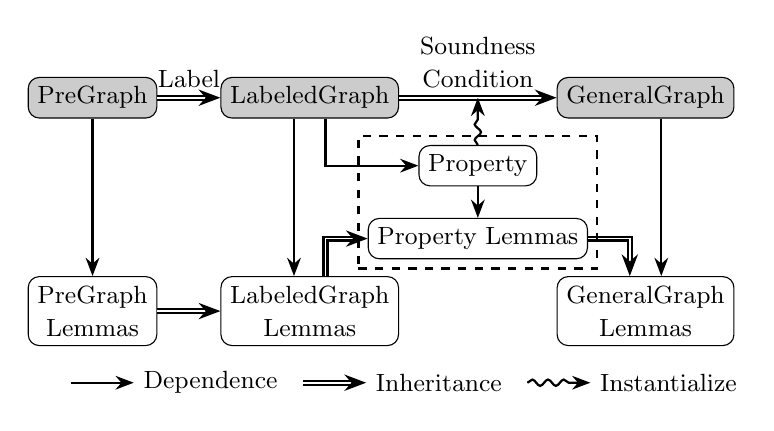
\begin{tikzpicture}
[->/.style={thick,arrows={-Stealth}},
-->/.style={thick,arrows={-Stealth}, decorate, decoration={snake, amplitude=.4mm,segment length=2mm,post length=2mm}},
   realG/.style={shape=rectangle, rounded corners=4pt, draw, fill=gray!40},
   propG/.style={shape=rectangle, rounded corners=4pt, draw}]
\node[realG] (PG) at (0, 0) {\small PreGraph};
\node[realG] (LG) [right=0.8 of PG] {\small LabeledGraph};
\node[realG] (GG) [right=2 of LG] {\small GeneralGraph};
\draw [double, ->] (PG) -- (LG) node [pos=0.5, above] {\small Label} ;
\draw [double, ->] (LG) -- (GG) node (SC) [pos=0.5, above, align=center]
{\small Soundness \\ \small Condition};
\node[propG] (Prop) [below=0.6 of SC] {\small Property};
\node[propG] (PropL) [below=0.4 of Prop] {\small Property Lemmas};
\node[propG] (PGL) [below=2 of PG, align=center] {\small PreGraph \\\small Lemmas};
\node[propG] (LGL) [below=2 of LG, align=center] {\small LabeledGraph \\\small Lemmas};
\node[propG] (GGL) [below=2 of GG, align=center] {\small GeneralGraph \\\small Lemmas};
\draw [double, ->] (PGL) to (LGL);
%% \draw [double, ->] (LGL) to (GGL);
\draw [->] (PG) to (PGL);
\draw [->] (Prop) to (PropL);
\draw [-->] (Prop) to (SC);
\coordinate [left=0.2 of LG.south] (LGs1);
\coordinate [left=0.2 of LGL.north] (LGLn1);
\draw [->] (LGs1) to (LGLn1);
\coordinate [right=0.2 of LG.south] (LGs2);
\coordinate [right=0.2 of LGL.north] (LGLn2);
\draw [->] (LGs2) |- (Prop);
\draw [double, ->] (LGLn2) |- (PropL);
\coordinate [right=0.2 of GG.south] (GGs);
\coordinate [left=0.2 of GGL.north] (GGLn1);
\coordinate [right=0.2 of GGL.north] (GGLn2);
\draw [double, ->] (PropL) -| (GGLn1);
\draw [->] (GGs) to (GGLn2);
\node [draw, thick, rectangle, dashed, fit=(Prop) (PropL)] {};
\node (legend1) [below right=0.2 and -0.3 of PGL] {\small Dependence};
\coordinate[left=0.8 of legend1]  (l1);
\draw [->] (l1) to (legend1);
\node (legend2) [right=1 of legend1] {\small Inheritance};
\coordinate[left=0.8 of legend2]  (l2);
\draw [double, ->] (l2) to (legend2);
\node (legend3) [right=1 of legend2] {\small Instantialize};
\coordinate[left=0.8 of legend3]  (l3);
\draw [-->] (l3) to (legend3);
\end{tikzpicture}
\endpgfgraphicnamed
\vspace{1ex}
\caption{Structure of the Mathematical Graph Library}\label{fig:graphs}
\end{figure}

\begin{figure}[t]
\centering
\beginpgfgraphicnamed{pregraphexp}
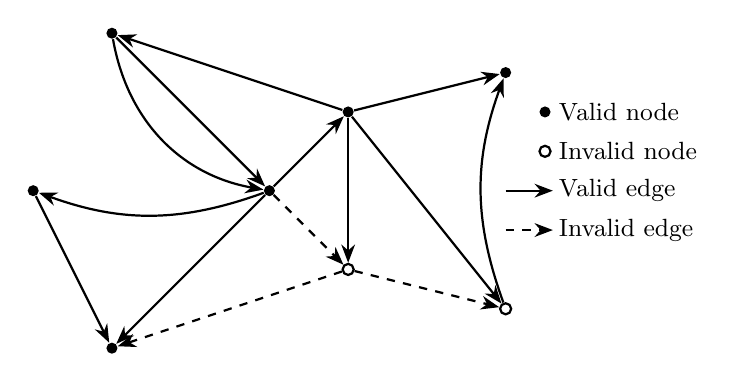
\begin{tikzpicture}
[vad/.style={circle, fill=black, inner sep=0pt, minimum size=4pt},
 inv/.style={circle, draw=black, thick, inner sep=0pt, minimum size=4pt},
 ->/.style={thick, arrows={-Stealth}}]
\node[vad] (n1) at (0, 0) {};
\node[vad] (n2) at (1, 1) {};
\node[inv] (n3) at (1, -1) {};
\node[vad] (n4) at (-2,2) {};
\node[vad] (n5) at (-2,-2) {};
\node[vad] (n6) at (-3,0) {};
\node[vad] (n7) at (3,1.5) {};
\node[inv] (n8) at (3,-1.5) {};
\node[vad] (n9) at (3.5, 1) {};
\node[inv] (n10) at (3.5, 0.5) {};
\node at (3.5, 1) [right=1.5pt] {\small Valid node};
\node at (3.5, 0.5) [right=1.5pt] {\small Invalid node};
\node at (3.5, 0) [right=1.5pt] {\small Valid edge};
\node at (3.5, -0.5) [right=1.5pt] {\small Invalid edge};
\draw[->] (n1) to (n2);
\draw[->,dashed] (n1) to (n3);
\draw[->,dashed] (n3) to (n5);
\draw[->] (n2) to (n3);
\draw[->] (n2) to (n7);
\draw[->] (n2) to (n8);
\draw[->,dashed] (n3) to (n8);
\draw[->] (n4) to (n1);
\draw[->] (n1) to (n5);
\draw[->] (n2) to (n4);
\draw[->] (n1) to [bend left=20] (n6);
\draw[->] (n6) to (n5);
\draw[->] (n8) to [bend left=20] (n7);
\draw[->] (n4) to [bend right=35] (n1);
\draw[->] (3.0, 0) -- (3.6, 0);
\draw[->,dashed] (3.0, -0.5) -- (3.6, -0.5);
\end{tikzpicture}
\endpgfgraphicnamed
\vspace{1ex}
\caption{A PreGraph with invalid nodes and edges.}\label{fig:pregraph}
\end{figure}

Figure~\ref{fig:graphs} gives the overall architecture of how our graphs are constructed.
The most basic kind of graph is PreGraph, out of which we build LabeledGraphs, and which in turn are used
to build GeneralGraphs.  Each kind of graph has some associated lemmas, and each kind inherits the lemmas of the previous kind.  The dashed box represents a ``plugin'' system for attaching arbitrary properties to LabeledGraphs and will be discussed more later. %We will consider each in turn.

\paragraph{Pregraphs.} A PreGraph is a hextuple $(V, E, \phi_V, \phi_E, s, t)$,
where $V$ and $E$ are the underlying carrier set of vertices and edges.  Not every $v \in V$ or $e \in E$ is actually ``in'' the graph, so we provide the predicates $\phi_V$ and $\phi_E$ to classify vertices and edges as \emph{valid} (in) or not (out).  Finally, $s$ and $e : E -> V$ are functions that map an edges to their source and destination respectively; this model means that PreGraphs are directed rather than undirected.  By design, there are no requirements for \emph{e.g.} how the validities of edges and vertices relate.  As shown in Figure \ref{fig:pregraph}, a PreGraph can contain invalid nodes and edges in an arbitrary configuration.

The advantage of designing a graph type that can reason about missing vertices and edges is because some of our later definitions need such flexibility.  Consider the difference of two graphs, $\gamma_1 - \gamma_2$.  Even if both of these graphs are ``well-formed'' to begin with, in the sense that valid nodes have only valid edges and vice versa, their difference may not since there may be dangling edges pointing to the now-removed vertices of $\gamma_2$.

Many basic graph concepts such as \emph{path}, \emph{reachability}, and \emph{subgraph} are defined on PreGraphs.
Informally a path is a list of nodes connected by edges.  Formally it is more convenient to
define a path as an ordered pair $(n,l)$ where $n$ is a node and $l$ is a list of edges.
A valid path requires $n$ to be the source of the first edge of $l$ (if one exists) and moreover
requires $l$ to be ``well chained''.  That is, the destination of one edge in $l$ must be the 
source of the next edge.  The list $l$ can be null to represent an empty path starting and ending
at the node $n$.  We prefer this encoding as opposed to some others (\emph{e.g.} a list of edges)
because the definitions of important concepts like reachability are cleaner.

The most important definition on PreGraph is the concept of reachability.
We use the notation $\gamma \models L_{n_2}^{n_1}(P)$ to mean that we can reach $n_2$ from $n_1$ via the path $L$ in PreGraph $\gamma$, and moreover that every node in $L$ satisfies predicate $P$.  This notation, along
with some derived ones such as
\begin{equation*}
\begin{split}
\gamma\models n_1 \xrightarrow{P} n_2 &\defeq \exists L, \gamma \models L_{n_2}^{n_1}(P),\\
\gamma\models n_1 \leadsto n_2 &\defeq \exists L, \gamma \models L_{n_2}^{n_1}(True)
\end{split}
\end{equation*}
form the bedrock of nearly every nontrivial predicate about and relation between
graphs.
We write $\p{reachable}(\gamma,v)$ to mean the set of vertices reachable in $\gamma$ from a given vertex $v$.

In \S\ref{sec:spacegraph} we will tie mathematical graphs $\gamma$ to a spatial graph predicate
$\p{graph}(x, \gamma)$.   As we will see, $\p{graph}$ ``owns'' only the
spatial portion of $\gamma$ that is reachable
from $x$ even though $\gamma$ may contain other nodes.  Accordingly, when we reason about
$\p{graph}(x, \gamma)$, it is natural to want to describe the
reachable portion of $\gamma$.  In fact we generalize this
idea into two concepts: the subgraph of $\gamma$ satisfying
an arbitrary predicate $P$, written $\gamma \!\downarrow\! P$, and the \emph{relaxed subgraph}, written $\gamma \!\uparrow\! P$, which contains the all of the subgraph plus some additional edges.  In particular, $\gamma \!\downarrow\! P$ contains exactly the vertices satisfying $P$ and only the edges whose source and destination both satisfy $P$.  The relaxed subgraph $\gamma \!\uparrow\! P$ adds the additional edges whose \textbf{source} satisfies $P$, even though their destination may not.
We can use these definitions to, for example, extract the subgraph or relaxed subgraph reachable from a vertex $v$ by writing \emph{e.g.}
\[
\gamma \!\downarrow\! (\lambda v'. \gamma\models v \leadsto v')
\]

\paragraph{LabeledGraph.} 
PreGraph and its derived properties (reachability, subgraph, etc) are
inadequate for real program verification, even though many basic lemmas can already be proved about them.
However, when reasoning about the concrete graphs manipulated by various algorithms, 
we usually need to add a notion of \emph{labels} on vertices and/or edges, such as
the ``mark bit'' used in Figure~\ref{fig:markgraph}.

\paragraph{GeneralGraph.}
Much more interesting is the concept of GeneralGraph, which augments a LabeledGraph by adding a user-specified soundness condition.  In Figure~\ref{fig:graphs} this soundness condition is highlighted by a dashed border.  These ``plugins'' can specify many different kinds of properties.  Each property, in turn, can be used to prove many property-specific lemmas, all of which then apply to the instantiating GeneralGraph.

\subsection{Graph plugins}

Many theorems about graphs require certain properties, such as:
\begin{itemize}
\item A graph may be finite (\p{FiniteGraph}), meaning that both the set of valid vertices and the set of valid edges are finite.
\item A less restrictive property is \emph{locally finite} (\p{LocalFiniteGraph}), in which each vertex has a finite number of neighbors.  Locally finite graphs are useful, for example, when we wish to reason about algorithms that process vertices by cycling through neighbors, such as breadth-first search.
\item More subtly, consider that many real data structures use special null values to represent unused edges.  The \p{MathGraph} property introduces this concept---\emph{i.e.} some invalid nodes that are none-the-less allowed to appear as destinations for valid edges.
\item Many of our verified algorithms have only two outgoing edges per node.  The \p{BiGraph} property lets us reason about this common special case in a convenient manner.
\end{itemize}
We have a number of other properties in our codebase, but these four are the most important basic ones.

\begin{figure}[t]
\centering
\beginpgfgraphicnamed{graphproperty}
\begin{tikzpicture}
[->/.style={thick,arrows={-Stealth}},
   group/.style={shape=rectangle, draw, thick, dashed},
   propG/.style={shape=rectangle, rounded corners=4pt, draw}]
\node[propG] (PL12) at (0, 0) {\small Lemmas of Property 1 and 2};
\coordinate [left=1 of PL12.north] (PL12n1);
\coordinate [right=1 of PL12.north] (PL12n2);
\node[propG] (PL1) [above=0.5 of PL12n1, align=center] {\small Property 1 \\\small Lemmas};
\node[propG] (PL2) [above=0.5 of PL12n2, align=center] {\small Property 2 \\\small Lemms};
\node[propG] (P1) [above=0.5 of PL1] {\small Property 1};
\node[propG] (P2) [above=0.5 of PL2] {\small Property 2};
\draw [->] (P1) to (PL1);
\draw [->] (P2) to (PL2);
\draw [double, ->] (PL1) to (PL12n1);
\draw [double, ->] (PL2) to (PL12n2);
\draw [->] (P1.west) to [bend right=45] (PL12.west);
\draw [->] (P2.east) to [bend left=45] (PL12.east);
\node (R1) [group, fit=(P1) (PL1)] {};
\node (R2) [group, fit=(P2) (PL2)] {};
\node (R3) [group, fit=(current bounding box)] {};
\node [propG] (P1P2) [above right=-1.1 and 1.2 of R3, align=left] {\small Property 1$/|$ \\\small Property 2};
\node [propG] (PL1PL2) [below=0.5 of P1P2, align=center] {\small Prop. 1 Lemmas \\\small Prop. 2 Lemmas \\\small Prop. 1$/|$2 Lemmas};
\draw [->] (P1P2) to (PL1PL2);
\node (R4) [group, fit=(P1P2) (PL1PL2)] {};
\node (EQ) [right=0 of R3] {\bf \Large $\mapsto$};
\end{tikzpicture}
\endpgfgraphicnamed
\vspace{1ex}
\caption{Combining plugins}\label{fig:properties}
\end{figure}

We use Coq's typeclass system to manage our plugins in a smooth manner.  Essentially the typeclass system enables the diagram in Figure~\ref{fig:properties}.  The idea is that if we have two properties, each of which come with some already-proved lemmas, we can combine these plugins to prove the emergent lemmas that result from the combination, and then treat the new combination as a new plugin.  Since the system is compositional, we can easily mix many different properties together.  For example, we compose \p{BiGraph}, \p{MathGraph}, and \p{FiniteGraph} together into a new plugin we call \p{BiMaFin}.  \p{BiMaFin} is the actual soundness condition used to verify the program in Figure~\ref{fig:markgraph}.

One interesting example of this process is the following lemma:
\newtheorem{mylem}{Lemma}
\begin{mylem}[Computable reachability]\label{lem:computereach}
\[
\begin{split}
\forall \gamma, x.~&\p{MathGraph}\ \gamma => \p{LocalFiniteGraph}\ \gamma =>\\
        & \p{reachable}(\gamma, x)\textrm{ is finite} => \\
        & \text{we can \textbf{compute} a set }S \text{ s.t.\ } \\
        & \quad \forall v.~v \in S <=> \gamma \models x \leadsto v.
\end{split}
\]
\end{mylem}
The proof of this lemma is a bit subtle.  To compute the reachable set
we need to design a decision procedure that explores the (potentially cyclic)
graph.  Accordingly we implement a flavor of breadth-first search, also keeping
track of the nodes that we have explored previously.  Since nodes are explored
in BFS order while reachability is in some sense defined in DFS order, when
we reach a node $n$ we must take some care to reconstruct a path from the origin to $n$
to satisfy the reachability property.  The definition is also
painful because of Coq's insistence that all computations terminate; we 
utilized the techniques outlined by Chlipala to pacify Coq's termination checker~\cite{chlipala:cpdt}.
 
\subsection{Reasoning about relations between graphs} %Using our framework to reasonApplication of the framework}

We apply our framework to define other structures and relations
between these structures (including graph), and then use them to prove
certain pure facts proposed by real verifications.

For example, we define DAG (directed acyclic graph) as a PreGraph with
an additional property: forall any $x$ and $y$, if $x$ is reachable
from $y$, then $x = y$ or $y$ is not reachable from $x$.  Similarly, we define tree 
by saying that for any reachable node $n$ there is a unique path from the root
to $n$.

We already defined the relation $\m{mark}(\gamma, \tx x, \gamma')$, used in 
the graph marking algorithm, in Figure~\ref{fig:markgraph}.  
Similarly, we define $\m{span}$ for the spanning tree program
and $\m{copy}$ for the graph copy program.  These relations all
capture how the graph has changed from before to after the program 
execution.  As previously mentioned, we reuse $\m{mark}$ and its
related lemmas to prove facts about spanning tree and graph copy 
because the latter two programs mark nodes as they work. 
Accordingly, we can reuse the following fact:
\begin{equation*}
\begin{split}
\forall \gamma, x, n.~&\gamma(x)=(0, v_1, v_2,\dots,v_n) => \m{mark1}(\gamma, x, \gamma_1) =>\\
        & \m{mark}(\gamma_1,v_1,\gamma_2) => \m{mark}(\gamma_2,v_2,\gamma_3) => \dots =>\\
        & \m{mark}(\gamma_n,v_n,\gamma_{n+1}) => \m{mark}(\gamma,x,\gamma_{n+1}).
\end{split}
\end{equation*}
This is a general theorem for any \p{LocalFiniteGraph}, not just
\p{BiGraph}. In our framework, we aspire to prove theorems as generally as possible.



\section{Defining and reasoning about spatial graphs}
\label{sec:spacegraph}
To prove the functional correctness of graph-manipulating algorithms implemented in a real language, we need to connect the heap representation of graphs, the memory model of the programming language, and the mathematical properties of graphs from \S\ref{sec:mathgraph}.  The first of these turns out to be surprisingly subtle as we shall see in \S\ref{sec:fixpointfail} and \S\ref{sec:goodgraph}.  The main challenge for the others is to engineer a framework that is generic enough and modular enough to be useful in practice in a variety of settings; we cover it in~\S\ref{sec:ramifylib}.

\subsection{Recursive definitions yield poor \p{graph} predicates}\label{sec:fixpointfail}

\newcommand{\graphkt}{\p{graph}_T}
\newcommand{\grapham}{\p{graph}_A}

Recursive predicates are ubiquitous in separation logic---so
much so that when a person writes the definition of a predicate as
\mbox{$P$ ``$\defeq$'' $\ldots P \! \ldots$}, no one raises an eyebrow despite the
dangers of circularity in mathematics. Indeed, the vast majority of the time there
is no danger thanks to the magic of the Knaster-Tarski fixpoint
$\mu_{\mathsf{T}}$ \cite{tarski:fixpoint}.  Formally what is going on
is instead of defining $P$ directly, one defines a functional
\mbox{$F_P \defeq \lambda P.~ \ldots P \! \ldots$} and then defines $P$ itself as
\mbox{$P \defeq \mu_{\mathsf{T}} \, F_P$}.  Assuming (as one typically does
without comment) that $F_P$ is \emph{covariant}, i.e. $(P \vdash Q)
\Rightarrow (F \, P \vdash F \, Q)$, one then enjoys the fixpoint
equation $P \Leftrightarrow \ldots P \ldots$, formally justifying
typically written pseudodefinition (``$\defeq$'').

%Definition corec {B A: Type}  (F: (B -> pred A) -> (B -> pred A)) : B -> pred A :=
%fun x w => forall P: B -> pred A, (forall x, F P x |-- P x) -> P x w.

Suppose we define a graph predicate $\graphkt$ this way, \emph{e.g.} along the lines of the fold/unfold definition in Figure~\ref{fig:markgraph}: %, \emph{i.e.}
\vspace{-1ex}
\[
\begin{array}{@{}l@{}l@{}}
\graphkt(x, \gamma) \stackrel{\Delta}{=} & (x = 0 /| \p{emp}) |/ \null \\
& \exists m,l,r.~ \gamma(x)=(m,l,r) /| \null \\
& ~~  x |-> m,l,r ** \graphkt(l, \gamma) ** \graphkt(r, \gamma)
\end{array}
\vspace{-1ex}
\]
%We have removed the alignment-related portions of equation~\eqref{eqn:bigraphintrofoldunfold} to focus on a more serious issue, even though as we will explain in~\S\ref{sec:goodgraph} alignment concerns are also necessary for the fold/unfold relationship to hold in C-like memory models.
The functional needed to define $\graphkt$ is covariant, so we can apply Knaster-Tarski; however, the result is hard to use.

Consider the following memory $m$ for a toy machine:

\begin{minipage}{.24\textwidth}
\qquad \[
\begin{array}{l|l}
\textrm{address} & \textrm{value} \\
\hline
102 & 0 \\
101 & 100 \\
100 & 42 \\
\end{array}
\]
\end{minipage}
\begin{minipage}{.19\textwidth}
\centering
\beginpgfgraphicnamed{selfref}
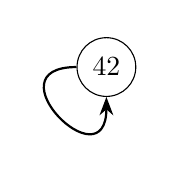
\begin{tikzpicture}
[->/.style={thick,arrows={-Stealth}},
   propG/.style={shape=circle, draw}]
   \path[use as bounding box] (-1, -1) rectangle (0.5, 0.5);
   \node[propG] (P) at (0, 0) {42};
   \draw[->] (P.west) .. controls (-1.5, 0) and (0, -1.5) .. (P.south);
\end{tikzpicture}
\endpgfgraphicnamed
\end{minipage}
\vspace{0.75ex}

\noindent Clearly $m |= 100 |-> 42,100,0$.  But it seems also clear that this memory represents a one-cell cyclic graph as illustrated in the accompanying diagram, \emph{i.e.} we want $m |= \graphkt(100,\hat{\gamma})$, where $\hat{\gamma}(100) = (42,100,0)$.  This is equivalent to wanting to be able to prove $100 |-> 42,100,0 |- \graphkt(100,\hat{\gamma})$.  Unfortunately, as hinted in Appendix~C\hide{\ref{apx:problemrecgraph}}, this seems rather difficult to do so since applying the natural proof techniques actually strengthen the goal.  In fact we do not know if this entailment is provable or not, but the difficulties encountered in proving what ``should be'' straightforward suggest that Knaster-Tarski should be treated with caution when defining spatial predicates for graphs.

The other direction, \mbox{$\graphkt(100,\hat{\gamma}) |- 100 |-> 42,100,0$},
\textbf{is} true but is not easy to prove, relying on the constructions in \S\ref{sec:goodgraph} and the fact that $\mu_{\mathsf{T}}$ constructs the least fixpoint.  In contrast, $\graphkt(100,\hat{\gamma}) |- 100 |-> 42,100,0 * \top$ is easy. % to prove. % via fold/unfold.

%As explained in~\S\ref{sec:foldunfold}, this alignment is necessary in C-like memory models to prove fold-unfold \eqref{eqn:bigraphintrofoldunfold}, which is why \eqref{eqn:bigraphintrofoldunfold} includes an alignment restriction $x~\mathsf{mod}~16 = 0$ and an existentially-quantified ``blank'' second field for the root $x \mapsto m,-,l,r$.

%As shown in (\ref{eqn:bigraphintrofoldunfold}) of Section
%\ref{sec:orientation}, Hobor and Villard\cite{hobor:ramification}
%defined the separation logic graph predicate
%$\mathsf{graph}(x,\gamma)$ in direct analogy to the standard
%separation logic definition of a tree. Note that the two-neighborhood
%means $\gamma$ is a BiGraph. However, it is peculiarly challenging in
%rigorously formalizing $\p{graph}$.

%* Showing that neither traditional fixpoint method works

%Appel and McAllester proposed another fixpoint $\mu_{\mathsf{A}}$
%that is sometimes used to define recursive predicates in separation
%logic \cite{appel:fixpoint}.  This time the functional $F_P$ needs to be
%\emph{contractive}, which to a first order of approximation means that
%all recursion needs to be guarded by the ``approximation
%modality''~$\rhd$~\cite{appel:vmm}, \emph{i.e.} our graph predicate would
%look like
%\begin{align*}
%\grapham(x, \gamma) ~ &\stackrel{\Delta}{=}\\
% (x = 0 /| \p{emp}) & |/ \exists m,l,r.~ \gamma(x)=(m,l,r) /| \null \\
% x |-> m,l,r & ** \rhd \grapham(l, \gamma) ** \rhd \grapham(r, \gamma)
%\end{align*}
%
%Unfortunately, $\rhd P$ is not precise for all $P$, so $\grapham$ is not precise either.  The approximation modality's universal imprecision has never been noticed before. % in the literature.  %We must do better.

%%%%%%%%%%%%%%%%%%%%%%%%%%%%%%%%%%%%%%%%%%%%%%%%%%
%%%%%% Edit0: cut down contractive recursion
%%%%%%%%%%%%%%%%%%%%%%%%%%%%%%%%%%%%%%%%%%%%%%%%%%

\subsection{Defining a good \p{graph} predicate}\label{sec:goodgraph}

Rather than trying to define \p{graph} as a recursive fixpoint, we will instead give it a flat structure.  Graphs in separation logic have been defined in similar ways before~\cite{ilya-graphs}; what is new here is that we prove---with the amount of precision required to convince Coq---that we can still enjoy fold/unfold with our definition.  Our path starts with the iterated separating conjunction or ``big star'', defined as:
%%%%%%%%%%%%%%%%%%%%%%%%%%%%%%%%%%%%%%%%%%%%%%%%%%
%%%%%% Edit1
%%%%%%%%%%%%%%%%%%%%%%%%%%%%%%%%%%%%%%%%%%%%%%%%%%
%%%%%% Edit1: Qinxiang's proposal starts
%%%%%%%%%%%%%%%%%%%%%%%%%%%%%%%%%%%%%%%%%%%%%%%%%%
\iftrue
\[
\begin{array}{@{}l@{}}
\underset{\{l_1, l_2,\dots,l_n\}}{\bigstar}P ~~ \defeq ~~ P(l_1) *
  P(l_2) * \dots * P(l_n) \\
\underset{S}{\bigstar} P ~~ \defeq ~~ \exists L.~ (\p{NoDup}\ L) /| (\forall x.~ x\ \p{in}\ L <=> x \in S) /| \underset{L}{\bigstar}P
\end{array}
\]
Big star $\bigstar$ is first defined over a list and then extended to sets.  We are now ready to define a good \p{graph} predicate:
\fi
%%%%%%%%%%%%%%%%%%%%%%%%%%%%%%%%%%%%%%%%%%%%%%%%%%
%%%%%% Edit1: Qinxiang's proposal ends
%%%%%%%%%%%%%%%%%%%%%%%%%%%%%%%%%%%%%%%%%%%%%%%%%%
%%%%%% Edit1: Original version starts
%%%%%%%%%%%%%%%%%%%%%%%%%%%%%%%%%%%%%%%%%%%%%%%%%%
\iffalse
\begin{equation*}
  \underset{\{l_1, l_2,\dots,l_n\}}{\bigstar}P ~~ \defeq ~~ P(l_1) *
  P(l_2) * \dots * P(l_n).
\end{equation*}
Formally $\bigstar$ is defined over a list rather than a set and is parameterized by a predicate $P$.  It is natural to extend $\bigstar$ to a set $S$ with an existentially-quantified duplicate-free list~$L$:
\[
\underset{S}{\bigstar} P ~~ \defeq ~~ \exists L.~ (\p{NoDup}\ L) /| (\forall x.~ x\ \p{in}\ L <=> x \in S) /| \underset{L}{\bigstar}P
\]
We use the same $\bigstar$ notation since the concepts are similar, but the existential adds a little pain since we need to prove that all choices of $L$ yield equivalent predicates.

We are now ready to give a good \p{graph} predicate:
\fi
%%%%%%%%%%%%%%%%%%%%%%%%%%%%%%%%%%%%%%%%%%%%%%%%%%
%%%%%% Edit1: Original version ends
%%%%%%%%%%%%%%%%%%%%%%%%%%%%%%%%%%%%%%%%%%%%%%%%%%
\vspace{-1.5ex}
\begin{equation}\label{eqn:iter_def}
  \p{graph}(x, \gamma) ~~ \defeq ~~ \underset{v \in \mathit{reach}(\gamma, x)}{\bigstar} v\mapsto\gamma(v)
\vspace{-1.5ex}
\end{equation}
$\gamma$ is a GeneralGraph and ``$x |-> \gamma(x)$'' is a predicate that says how a single node fits in memory; in Figure~\ref{fig:markgraph} it was:
\[
\exists m,l,r.~\gamma(x) = (m,l,r) /| x |-> m,-,l,r /| x\ \p{mod}\ 16 = 0
\]
$\gamma$ need not be a bigraph, but \emph{e.g.} can have many edges.

Our definition of \p{graph} is flat in the sense that there is no obvious way to follow the link structure recursively.  Happily, we can recover a general recursive fold/unfold (if $x |-> \gamma(x)$ and the GeneralGraph have the necessary properties):
\vspace{-1ex}
\begin{equation}
\label{eqn:unfold_graph}
\hspace{-1em}\begin{array}{@{}lc@{\hspace{1pt}}c@{\hspace{1pt}}l@{}}
\p{graph}(x,\gamma)  <=>  x |-> \gamma(x) ** \big(\!\!\!\!\!\!\!\!\!\!\!\!\!\underset{n \in \p{neighbors}(\gamma,x)}{\raisebox{-0.3ex}{\resizebox{0.75em}{!}{$\scon$}} \hspace{-2.18ex} \bigcup}\!\!\!\!\!\!\!\!\!\!\!\! \p{graph}(\gamma,n) \big) \\
[2pt]
\text{~~~ where ~~ }\underset{l_1,\dots,l_n}{\raisebox{-0.3ex}{\resizebox{0.75em}{!}{$\scon$}}\hspace{-2.18ex} \bigcup} \! \! P  \defeq  P(l_1) ** \ldots ** P(l_n) \end{array}
\vspace{-1ex}
\end{equation}

The proof of the $<=$ direction requires care. The difficulty is that if two nodes $x |-> \gamma(x)$ and $x' |-> \gamma(x')$ are \emph{skewed}, \emph{i.e.} ``partially overlapping'' with some---but not all---of $x$'s memory cells shared with $x'$, then the $\bigstar$ on the left hand side cannot separate them.  To avoid skewing we require $x |-> \gamma(x)$ be \emph{alignable}.  A predicate $P$ is alignable when
\[
\forall x,y.~ \Big(P(x) ** P(y) |- \big(P(x) /| x = y\big) |/ \big(P(x) * P(y)\big)\Big)
\]
That is, either they are completely on top of one another or they do not interfere at all.  In a Java-like memory model such as in HIP/SLEEK this property is automatic because pointers in such a model always point to the root/beginning of an object.  In contrast, in a C-like memory model such as in VST/CompCert, this property is not automatic because pointers can point anywhere.  In such a model, alignment is most easily enforced by storing graph nodes at addresses that are multiples of an appropriate size (16 in Figure~\ref{fig:markgraph}).

Some of our VST proofs do not use fold/unfold, instead preferring to use the lemmas in~\S\ref{sec:ramifylib} directly.  On the other hand, for HIP/SLEEK fold/unfold is vital, and knowing that the recursive relationship holds produces a pleasant feeling.  We also prove fold/unfold lemma for DAGs in which we get a $*$ between the root and its $\medocon$-joined neighbors. % rather than the $**$ present in \eqref{eqn:unfold_graph}.

\subsection{Ramification Libraries}\label{sec:ramifylib}

\begin{figure}[t]
\centering
\beginpgfgraphicnamed{infrastructure}
\begin{tikzpicture}[
->/.style={thick, arrows={-Stealth}},
ent/.style={shape=rectangle, rounded corners=4pt, draw, on grid}]
\node[ent] (SM) at (0, 0) {\small Step-Indexed Model};
\node[ent] (DM) [right=4.4 of SM] {\small Direct Model};
\node[ent] (CL) [above=1 of SM] {\small Core Logic};
\node[ent] (SL) [above=1 of DM] {\small Supplementary Logic};
\node[ent] (LF) [above left=1 and 1.2 of CL] {\small Logic Facts};
\node[ent] (RF) [above right=1 and 1.2 of CL] {\small Basic Ramification};
\node[ent] (BF) [above=1 of LF] {\small $\bigstar$ Facts};
\node[ent] (BR) [above=1 of RF] {\small $\bigstar$ Ramification};
\node[ent] (GF) [above=1 of BF] {\small Graph Facts};
\node[ent] (GR) [above=1 of BR] {\small Graph Ramification};
\node[ent] (SLF) [above=1 of SL] {\small Supplementary Logic Facts};
\node[ent] (SBF) [above=1 of SLF] {\small Supplementary $\bigstar$ Facts};
\node[ent] (SGF) [above=1 of SBF] {\small Supplementary Graph Facts};
\draw [double, ->] (SM) to (CL);
\draw [double, ->] (SM) to (SL);
\draw [double, ->] (DM) to (CL);
\draw [double, ->] (DM) to (SL);
\draw [->] (CL) to (LF);
\draw [->] (CL) to (RF);
\draw [->] (CL) to (SL);
\draw [->] (SL) to (SLF);
\draw [->] (SLF) to (SBF);
\draw [->] (SBF) to (SGF);
\draw [->] (LF) to (RF);
\draw [->] (LF) to (BF);
\draw [->] (RF) to (SLF);
\draw [->] (RF) to (BR);
\draw [->] (BF) to (BR);
\draw [->] (BF) to (GF);
\draw [->] (GF) to (GR);
\draw [->] (GR) to (SGF);
\draw [->] (BR) to (GR);
\draw [->] (BR) to (SBF);
\node (legend1) [below right=0.2 and -1.2 of SM] {\small Dependence};
\coordinate[left=0.8 of legend1]  (l1);
\draw [->] (l1) to (legend1);
\node (legend2) [right=1 of legend1] {\small Instantialization Choices};
\coordinate[left=0.8 of legend2]  (l2);
\draw [double, ->] (l2) to (legend2);
\end{tikzpicture}
\endpgfgraphicnamed
\vspace{1ex}
\caption{Infrastructure of ramification library}\label{fig:infra}
\end{figure}

We provide the architecture of our spatial development in Figure~\ref{fig:infra}.  Starting from the bottom, notice that there are two underlying heap models: the Step-Indexed Model, which is the main heap model used in VST, and a much simpler Direct Model, which is used by HIP/SLEEK among others.  The Step-Indexed model is much fancier, but none of our development depends on its bells and whistles.

To isolate our development from these unnecessary complications, and to ensure that HIP/SLEEK can reuse our spatial reasoning, we use two interfaces: Core Logic and Supplementary Logic.  Both models can instantiate both interfaces, but generally speaking our VST proofs only need the Core properties to prove our examples, whereas HIP/SLEEK uses both Core and Supplemental.  Each interface defines some operators of separation logic and provides some axioms about how they work.  For example, $*$ and $--*$ are in Core Logic, along with the axiom $(P |- Q --* R) <=> (P * Q |- R)$.  On the other hand, the $**$ and $--o$ operators are in Supplementary Logic, along with rules like $P |- P ** P$.

Above the Logic layer we have three towers, each three levels high.  The leftmost tower contains basic lemmas about Logic, $\bigstar$, and \p{graph}.  In the $\bigstar$ Facts box we prove \emph{e.g.}:
\[
\infrule{}
{A \cap B = \emptyset}
{\underset{x\in A}{\bigstar} P(x) *   \underset{x\in B}{\bigstar} P(x) \Leftrightarrow \underset{x\in A \cup B}{\bigstar} P(x)}{}
\]

The middle tower is more interesting in that it is entirely focused on ramification entailments.  A robust library of ramification entailments is essential to make ramification work smoothly in practice.  The lowest level contains lemmas like:
\[
%\infrule{Ramify-Q-SPLIT}
\infrule{}
{G_1 \vdash L_1 * \forall x.~ (L_2 --* G_2) \\
 G'_1 \vdash L'_1 * \forall x.~ (L_2' --* G'_2)}
{G_1 * G'_1 \vdash (L_1 * L'_1) * \forall x.~ \big((L_2 * L'_2)--* (G_2 * G'_2)\big)}{}
\]
We use this lemma to break large ramification entailments into more manageable pieces in a compositional way. % compositionally.

The middle level contains $\bigstar$ ramification lemmas, \emph{e.g.}:
\begin{equation}
\label{ramify:bigstar}
\infrule{}
{A \cap B = \emptyset  \qquad  A' \cap B = \emptyset}
{\underset{x\in A\cup B}{\bigstar} P(x) \vdash \! \underset{x\in A}{\bigstar} \! P(x) * \Big( \underset{x\in A'}{\bigstar} \! P(x) \! \wand \! \! \! \! \underset{x\in A' \cup B}{\bigstar} \! \! P(x)\Big)}{}
\end{equation}

The top level is focused on graph ramifications, such as the following ``update one node'' lemma:
\begin{equation}
\label{lem:updategraphnode}
%{\gamma(x_0) = \gamma'(x_0) \text{ for any } x_0 \neq x }
\infrule{}
{\forall x_0 \neq x.~ \gamma(x_0) = \gamma'(x_0) \\ \p{neighbors}(\gamma,x)=\p{neighbors}(\gamma',x)}
{\p{graph}(x, \gamma) \! \vdash \! x \! \mapsto \! \gamma(x) \! * \! \big(x \! \mapsto \! \gamma'(x) \! \wand \! \p{graph}(x, \gamma')\big)}{}
\end{equation}
This lemma was used on line~\ref{code:markram2} in Figure~\ref{fig:markgraph}.

This layered structure enables proof reuse. All of the theorems for $\p{graph}$ are proved from the properties of iterated separating conjunction, but having a modular library allows $\bigstar$ to be reused in other structures smoothly.

Also, all of our verifications of different graph algorithms use the proof rules of $\p{graph}$ at the top level in the library. Taking the marking algorithm we introduced in \S\ref{sec:orientation} as an example, we prove the following theorem from the library:
\begin{equation}
\label{lem:updatesubgraph}
\infrule{}
{n \in \p{neighbors}(\gamma,x)}
{
\mbox{
$\begin{array}{@{}l@{}l@{}}
\p{graph}(x, \gamma) \vdash \\
\p{graph}(n, \gamma) \! * \!
\big(\forall \gamma'. & \m{mark}(\gamma, n, \gamma') \! /| \! \p{graph}(n, \gamma') \! --* \null \\
& \m{mark}(\gamma, n, \gamma') \! /| \! \p{graph}(x, \gamma')\big)
\end{array}$
}
}{}
\end{equation}

The Supplementary tower contains properties not used by most of the VST examples.  This includes the fold/unfold relationship from \S\ref{sec:goodgraph}, facts about precision, and so forth.  Some of these properties are needed by HIP/SLEEK, while others are mostly included for esthetic effect.

% are there just because we felt they might be useful in the future.

%One benefit of the definition in (\ref{eqn:iter_def}) is that the pure
%mathematical graph $\gamma$ in $\mathtt{graph}$ is not necessarily a
%BiGraph. (\ref{eqn:iter_def}) can represent a general graph with
%variant number of neighors as long as extending the definition of
%$\gamma(x)$ to data mapped by the label function and every neighbor of
%node $x$.
%
%Moreover, it turns out that the $\bigstar$ notation is a more useful
%and fundamental concept than $\mathtt{graph}$. There are two parts of
%the $\bigstar$ in (\ref{eqn:iter_def}): one is the predicate $\mapsto$
%and the other is the node set which the $\mapsto$ iterates on. They
%both bind to $\gamma$ in (\ref{eqn:iter_def}) for $\p{graph}(x,
%\gamma)$, which is a special case. In section \ref{sec:applicable}, we
%will see the specification of a spanning tree algorithm which uses
%$\bigstar$ directly instead of $\p{graph}$ because in that
%specification, the predicate $\mapsto$ and the node set bind to
%different mathematical graphs. Furthermore, we generalize the
%ramification rules for $\p{graph}$ in \cite{hobor:ramification}, which
%uses $\bigstar$ so as to be applied in all verification examples.

%% 1.2. \texttt{Iter\_sepcon} and \texttt{pred\_sepcon} are defined. And related ramification rules are proved.
%% 1.3. The most general graph-spatial-predicate \texttt{vertices\_at} are defined (for all possible styles of graphs). Related ramification rules are proved. Graph and graphs are defined as special cases of vertices at.

%% 2. A minor implementation trick. There are many tactics defined in \texttt{msl\_ext/ramify\_tactics.v}, which can manipulate low level heaps efficiently.

%% * Separating the material into the general vs. tool-specific part.  Measurements of etc.


\section{Certifying a Garbage Collector for CertiCoq}
\label{sec:certigc}
In this section, we explain how we used our graph library
to verify a generational copying garbage collector for the 
CertiCoq compiler. The GC is our most complicated example,
and we will discuss some of its key proofs, but the larger
point here is that we completed this certification using 
exactly the framework and the principles we have discussed
thus far. {\color{magenta}We enjoyed significant code 
reuse from our prior certifications, and when we stated 
new lemmas for the GC, we filed them away at the appropriate
``layers'' so that they may be reused in the future.}

% The last line above is currently false.
% We cannot edit the code to make it 100% true, 
% but the plan is to incorporate GCGraph's special
% properties into a soundness condition that will be
% added atop a LiMaFin-type LabeledGraph.
% Having done that, I'll weaken the last line
% above to match the actual work.

\subsection{Background}
\label{sec:gcbackground}

% My goal here is to start with a broad overview
% and then work my way down to forward
% at the end of this subsection I want it to be pretty
% clear that the whole game is just a series of calls
% to forward.
% This will set us up nicely for the decorated proof of
% forward in the next subsection.

The CertiCoq Project compiles Gallina code into CompCert 
C light, and then uses CompCert to compile C light
into assembly. In order to support Gallina's presumption of
infinite heap memory, CertiCoq provides garbage collection at
the C light level. Their generational copying garbage 
collector is written in C light, and is realistic, 
supporting variable-sized words, 12 generations... 
% Leaving this slot open for the time being, so
% we can highlight those features that we will discuss 
% the most in the technical part later.
Since CertiCoq aims to be end-to-end certified, the GC 
also needs certification.

The GC's client program, also called the mutator, controls
an array of arguments that it cares about. 
% Looking for better term than "cares about"
These arguments may point at memory blocks 
in the heap, and, recursively, the items in those
memory blocks may point at other blocks in the heap. 
By maintaining direct and indirect links to
blocks via this internal ``web of care'', 
% I'm a little iffy about introducing this additional
% analogy, but then again I don't want to introduce
% the analogy of a graph right away. That could be seen
% as a huge conceptual leap, and a skipped step. 
the mutator indicates that it 
cares about those blocks, and reserves the right to 
access them for reading or writing. 
% Maybe add a line about how the mutator can "drop"
% a block, thus showing that it won't need it anymore?

When the mutator runs out of heap space, 
it calls the garbage collector to free up memory. 
The GC is allowed to modify the heap as
it sees fit, with the condition that it not damage the 
mutator's web of care. By this we mean that the same items 
should be accessible from the mutator's arguments
array before and after the collection, and they 
should be reached from the arguments array by 
following similar links as before. 
Other features of the original web, such as where 
items were situated in the heap, may be changed. 
In SECTION, we will explain how we abstracted this
web into a mathematical graph, where preserving the 
web of care is analogous to showing graph isomorphism.

``We thus say that the arguments array is owned by the 
mutator, but the heap is owned by the GC.''

\subsection{Structure of the Program}
\label{sec:gcstructure}
% maybe a diagram showing how everythign calls forward? 
% I sketched one before, can show you sometime.
Ours is a generational copying garbage collector, which
means that it leans on the empirical observation that
new blocks often need to be collected soon after their
allocation, while blocks that survive this initial
culling tend to live for much longer.
% Hm, it would take about another 100 words to explain 
% this fully. I'm wondering if we can elide it, 
% treating the above as adequate revision, and assuming 
% they know the rest of the story.

The mutator only ever allocates new memory in the first, 
smallest generation of heap. This generation is thus 
called the nursery. On finding that the nursery is full, 
the mutator calls the garbage collector to free up space.
The main GC function triggers the collection of the nursery
into the second generation, which is twice in size. These generations
are called the \emph{from} and \emph{to} generations respectively.
To trigger a collection means to examine the elements 
in \emph{from}, see if they are accessible from the mutator's
args array either directly or indirectly, and, if they are, 
copy them over to \emph{to}. This copying is achieved over a few steps, 
and we will examine these shortly, but the larger picture is that 
everything of import in \emph{from} has been copied to \emph{to}, 
and so \emph{from} can safely be reset. The mutator will now have 
enough room for the allocation that it was trying to perform.

One subtlety in this discussion is that we enjoyed a 
guarantee that \emph{to} had enough room to accept 
\emph{from}'s items. In the (unlikely) worst case, 
\emph{all} of \emph{from}'s data was copied over to \emph{to}, 
so in other words \emph{to} could not have been more than 
half full. We relied on this guarantee before this collection, 
and we must ensure we will enjoy it the next time a collection 
is required. So, in case the collection of the nursery caused
the second generation to become more than half full, we trigger
a collection of the second generation to the third. This makes 
both the first and second generations empty, thus giving us our 
guarantee trivially. It should be 
clear to see that this may also trigger further collections in 
a cascade effect. 

Armed with an understanding of how the overall collection 
works, we move one level deeper and examine how we identify and 
copy those items in a \emph{from} generation that are reachable
from the args array tot he \emph{to} generation.

% 150 or so words that explain forward_roots and do_scan.
% End goal is to convince them that everything relies on forward, 
% and forward is all that remains to be explained.
% I can do this writing, just taking a break.

\subsection{Forward}
\label{sec:gcforward}
The Garbage Collector's main workhorse is the function \emph{forward}.
Given a pointer to a block that is in the \emph{from} generation, 
it makes a copy of that block in the \emph{to} generation.
{\color{blue}Maybe at this point we could dedicate one or 
two sentences to explaining that the whole dang opera is really just 
calls to \emph{forward}.}

Figure (blah) shows a decorated proof of the forward function.
The function's behavior is subtly different depending on 
whether the the pointer $p$ lives in the arguments array or in the 
heap itself. The difference lies in lines blah and blah, where 
we wish to update $p$ to point to the new forwarded block. 
When $p$ lives in the arguments array, this update is easy to 
reason about since $p$ is fundamentally $\bigstar$-separated from our heap. 
When $p$ is itself in the heap, this update itself constitutues a
write to the heap. In the decorated proof, we show the second 
case. To this end, we assume in line (blah) that p is (dododo). 

% for second branch
%$\left\{\!\!\!\begin{array}{l@{}} boo \end{array}\right\}$
% 
\begin{figure}[t]
\vspace{-1ex}
  \begin{lstlisting}
// $\left\{\!\!\!\begin{array}{l@{}} \forall \gamma, \m{f\_info}, \m{t\_info}, \m{outlier}, \m{from}, \m{to}, \m{forp}.~ \null \\ \p{gc\_graph}(\gamma) * \p{fun\_info}(\m{f\_info}, \m{fi}) * \p{thread\_info}(\m{t\_info}, \m{ti}) /| \null \\ \m{compat}(\gamma, \m{f\_info}, \m{t\_info}, \m{outlier}, \m{from}, \m{to}, \m{forp}) /| \null \\ \tx{from\_start} = \m{gen\_start}(\gamma, \m{from}) /| \null \\ \tx{from\_limit} = \tx{from\_start} + \m{gen\_size}(\gamma, \m{from}) /| \null \\ \tx{next} = \m{nextaddr}(\m{t\_info}, \m{to}) /| \null \\ \exists \m{v},\m{n}.~\m{forp}=(\m{v},\m{n}) /| \tx{p} = \m{vaddr}(\gamma, \m{v}) + \m{n}\end{array}\right\}$
void forward (value *from_start,
              value *from_limit,
              value **next,
              value *p,
              int depth) {
  value * v;
// $\searrow \left\{\!\!\!\begin{array}{l@{}} \tx{...} \tx{p} = \m{vaddr}(\gamma, \m{v}) + \m{n} /| \null \\ \exists \m{hd},\m{flds}.~ \m{hd} = \m{mkhd}(\gamma, \m{v}) /| \m{flds} = \m{mkfv}(\gamma, \m{v}) /| \m{v} |-> \m{hd},\m{flds} \end{array}\right\}$
// $\left\{\!\!\!\begin{array}{l@{}} \m{above} + \tx{p} = \tx{\&}(\m{flds}[\m{n}]) /| \m{iopi}(\tx{*p}) \end{array}\right\}$
  value va = *p; 
?? $\swarrow \{\m{line\_1} + \exists...~ /| \tx{va} = \m{flds}[\m{n}] /| \m{iopi}(\tx{va})\}$
// magic - we know that $\m{flds}[\m{n}]$ is an edge
// $\{\exists \m{e}, \m{v'}, \m{b}, \m{i}.~ \tx{va} = \m{flds}[\m{e}] = \m{vaddr}(\gamma, \m{dst}(\gamma, \m{e})) = \m{vaddr}(\gamma, \m{v'}) = \m{Vptr}(\m{b},\m{i})\}$
  if(Is_block(va)) {
    v = (value*)int_or_ptr_to_ptr(va);
// $\{\tx{v} = \m{Vptr}(\m{b},\m{i}) = \m{vaddr}(\gamma, \m{v'})\}$
// $\{(\m{Is\_from()} /| \tx{...}) \lor (\neg \m{Is\_from()} /| \tx{...})\}$
    if(Is_from(from_start, from_limit, v)) {
// $\searrow \left\{\!\!\!\begin{array}{l@{}} \exists \m{hd'},\m{flds'}.~ \m{hd'} = \m{mkhd}(\gamma, \m{v'}) /| \m{flds'} = \m{mkfv}(\gamma, \m{v'}) /| \m{v'} |-> \m{hd'},\m{flds'} \end{array}\right\}$
      header_t hd = Hd_val(v);
// $\swarrow \left\{\!\!\!\begin{array}{l@{}} \tx{hd} = \m{Z2val}(\m{hd'})  /| ((\tx{hd == 1}  /| tx{...}) \lor \null \\ (\tx{hd==0} /| \m{flds'}[0] = \m{vaddr}(\m{copvert}(\gamma, \m{v'}))))\end{array}\right\}$
      if(hd == 0) {
// $\searrow \left\{\!\!\!\begin{array}{l@{}} \exists \m{hd'},\m{flds'}.~ \m{hd'} = \m{mkhd}(\gamma, \m{v'}) /| \m{flds'} = \m{mkfv}(\gamma, \m{v'}) /| \null \\ \m{v'} |-> \m{hd'},\m{flds'} /| \m{flds'}[0] = \m{vaddr}(\m{copvert}(\gamma, \m{v'})) \end{array}\right\}$
        t = Field(v,0);
// $\swarrow \left\{\!\!\!\begin{array}{l@{}} \tx{t} = \m{vaddr}(\m{copvert}(\gamma, \m{v'})) \end{array}\right\}$
// $\searrow \left\{\!\!\!\begin{array}{l@{}} \exists \m{hd},\m{flds}.~ \m{hd} = \m{mkhd}(\gamma, \m{v}) /| \m{flds} = \m{mkfv}(\gamma, \m{v}) /| \null \\ \m{v} |-> \m{hd},\m{flds} /| \tx{p} = \tx{\&}(\m{flds}[\m{n}]) \end{array}\right\}$
        *p = t;
?? $\left\{\!\!\!\begin{array}{l@{}} \m{v} |-> \m{hd},(\m{upd\_nth}(\m{flds}, \m{vaddr}(\m{copvert}(\gamma, \m{v'}))))\end{array}\right\}$
// $\swarrow$ ??
// $\left\{\!\!\!\begin{array}{l@{}} \exists \gamma'.~ \p{uf\_graph}(\gamma') /| \gamma' = \m{lgd}(\gamma,\m{e},\m{copvert}(\gamma, \m{v'})) /| \null \\ \tx{postcondition}\end{array}\right\}$
      } else {
// remind them of old facts...
// $\{ \tx{hd} = \m{Z2val}(\m{hd'})\}$
        int i; int sz; value *new;
        sz = Wosize_hd(hd); new = *next+1; *next = new+sz;
// $\{\tx{sz} = \m{getvertsz}(\m{hd'}) = \m{lenflds}(\gamma, \m{v'}) /| \tx{new} = \m{sp\_start}(\m{to}) + \m{used}(\m{to}) + 1 /| \tx{??}\}$        
        Hd_val(new) = hd; // ??
        for(i = 0; i < sz; i++) {
          Field(new, i) = Field(v, i);
        }
        Hd_val(v) = 0;
        Field(v, 0) = ptr_to_int_or_ptr((void *)new);
// $\searrow$
        *p = ptr_to_int_or_ptr((void *)new);
// $\swarrow$
        if (depth>0)
        for (i=0; i<sz; i++)
          forward(from_start, from_limit, 
            next, &Field(new,i), depth-1);
      }
    }
  }
}
\end{lstlisting}

\vspace{-0.4em}
\caption{Clight code and proof sketch for forward}
\label{fig:forward}
\vspace{-1em}
\end{figure}

\subsection{Issues}
\label{sec:gccsemantics}

\paragraph{Pointer Subtraction.}
{\color{blue}Hmm I'm wondering if we should really be mentioning this,
strapped as we are for space. Anyway, will steal off your emails.}
\begin{figure}[t]
\vspace{-1ex}
  \begin{lstlisting}
if (h->spaces[i+1].start==NULL) {
  int w = h->spaces[i].limit-h->spaces[i].start;
  create_space(h->spaces+(i+1), RATIO*w);
}
\end{lstlisting}

\caption{Boundary Issues}
\label{fig:boundary}
\vspace{-1em}
\end{figure}

\paragraph{Double-Bounded Pointer Comparisons}









\section{Engineering our Techniques}
\label{sec:development}
\begin{table}[t]
\centering
\begin{tabular}{c|c|c}
Component & Number of files & Size (in lines)\\\hline
Math Graph (\S\ref{sec:mathgraph}) & 19 & 12,628\\
Spatial Graph (\$\ref{sec:spacegraph}) & 12 & 7,337 \\
Integration into Floyd (\S\ref{sec:vst}) & 12 & 1,917 \\
Modifications to H/S (\S\ref{sec:hipsleek}) & ~~51\tablefootnote{H/S files modified here is not necessarily fresh created.} & 2,500 \\
VST Examples (\S\ref{sec:application}) & 13 & 3,253 \\
H/S Example (\S\ref{sec:hipsleek}) & 2 & 429 \\
Memory Model \& Logic & 13 & 2,395 \\
Common Utilities & 10 & 3,085 \\\hline\hline
Total Development & 132 & 33,544 \\
\end{tabular}
\caption{Size of our codebase}
\label{tab:codebase}
\end{table}

All of our results in this paper have been machine-checked.  The vast bulk of our development was checked in Coq, although a 55-line file (shown in Figure~\ref{fig:hipmarkgraph}) was checked in HIP/SLEEK.  Our modifications to HIP/SLEEK itself were not machine-checked since HIP/SLEEK does not have a mechanized soundness proof.
Although the size of a development does not perfectly match with that development's importance or implementation difficulty, we present it nonetheless in Table~\ref{tab:codebase}, organized roughly by the paper section corresponding to each development.  It took fewer than 400 lines of Coq to verify the \li{mark} algorithm in HIP/SLEEK, indicating that a large portion of the codebase is shared between VST and H/S.

\hide{
\paragraph{Size of Coq mathgraph \S\ref{sec:mathgraph}.}
Graph folder has 18 files in total with 10,919 lines in total

\paragraph{Size of Coq spacegraph \S\ref{sec:spacegraph}.}

not including the connection to H/S or VST

include \li{Graph.v} and \li{GraphBi.v} from \li{msl_application} since they do not depend on the underlying VST model?

What is in \li{ramification_lemmas}?  %Any other parts of VST ``standard'' from our work?

\paragraph{Integration into Floyd (\S\ref{sec:vst}).}: ?
Size of additions to VST logic model: ?

\paragraph{Modifications to HIP/SLEEK.}
H/S code: approximately 2,500 lines of code across 51 files
Size of extra H/S memory model:
\li{alg_seplog_direct.v}  52 lines
\li{overlapping_direct.v} 442 lines  {\color{magenta}How do we handle alignment?}
\li{precise_direct.v} 111 lines
other files?

\paragraph{Size of VST examples~\S\ref{sec:application}.}

Note: graph, graphbi (in space), graphmark, graphbimark are shared in \li{msl_application}

mark graph  19 + 402 + 161 + 246 = 828
mark dag  19 + 402 + 161 + 210
Note: mark dag shares 19 + 402 + 161 with mark graph

copy   459 + 19 + 161 + 388 = 1,027 (need to add files from \li{msl_applicatin})
dispose   475 + 18 + 544 = 1,037 (need to add files from \li{data_structure})
What do copy or dispose share with mark or with each other?

total: 1,038 (marks) + 2,064 (copy/dispose, assuming no duplication) = 3,102 lines.  12 files, assuming no sharing for copy/dispose (with each other or with mark)

\paragraph{Size of H/S example.}
main file: 54 lines (Figure~\ref{fig:hipmarkgraph}), \li{Module Type} generated by H/S (Figure~\ref{fig:hipcoqfile}) is 30 lines, Coq \li{Module} matching this \li{Module Type} is 358 lines.
total: 2 human-generated files, 429 lines

\paragraph{Size of total development.} ?
}


\section{Related work}
\label{sec:related}
\section{Related and future work}

The most famous graph related theorem which has been mechanically
verified is the Four Color Theorem: Any planar map can be colored with
only four colours. In 2005, Benjamin Werner and Georges Gonthier
formalized a proof of the theorem \cite{gonthier2005computer} inside
Coq. It is very easy and natural to rephrase the problem in graph
theory: by taking regions as nodes and connecting each pair of
adjacent regions as edges, coloring the map is equivalent to coloring
the graph obtained. However, they used a different kind of
combinatorial structure, known as hypermaps, instead of
graphs. Basically, a hypermap is a type ``dart'' with several
functions mapping dart to dart. The combinatorial and geometrical
properties are encoded as certain permutation properties of those
functions. It is quite a very different structure from graph.

Lars Noschinski built a formalized graph library for the Isabelle/HOL
proof assistant and verified a method of checking Kuratowski subgraphs
used in the LEDA library. It supports general infinite directed graphs
with labeled and parallel arcs \cite{Noschinski2015}. His definition
of graph is similar to our PreGraph except he uses vertex/edge set
instead of validity functions. Besides, Noschinski's library also
covers basic graph related concepts such as reachable component and
spanning tree.

Nordhoff and Lammich \cite{Dijkstra_Shortest_Path-AFP} formalized and
proved Dijkstra's algorithm in Isabelle. Their graph is defined as
vertex and edge sets where the edge is a triple (source, label,
destination). They only defined what they need for the algorithm.

Written in HOL, Wong \cite{wong1991} expressed a small portion of the
conventional graph theory, which is mainly used to model the railway
track network and applied in signalling systems. It does not contain
too many graph property-related theorems.

Chou \cite{chou1994formal} formalized theory of undirected graphs in
HOL that emphasize on the notion and important properties of trees. He
applied this library to verified distributed algorithms
\cite{chou1995mechanical}.

Duprat \cite{duprat2001coq} 



5.2. An alternative way of verifying marking program is reasoning about the whole history of marking operations. The disadvantage of it is that it currently needs more work in a Hoare logic framework. The advantage of it is that its reasoning structure are more similar with the way we understand it in our first algorithm class.
5.3. I take some effort on garbage collector like graph structural. Though it is only connecting this special structural with 5.1.1 and 1.3, it takes much time and it is not finished yet.


\section{Future work and conclusion}
\label{sec:future}
\label{sec:conclusion}
As future work, we plan to improve the pure reasoning of graphs and
similar data structures. We also have plan to verify a garbage
collector algorithm of CertiCoq, which is a project focuses on a
certified compiler from Gallina to Clight. On HIP/SLEEK side, we tend
to use extensions to verify other kinds of code such as fast
exponentiation and more graph algorithms. We also have plan to make
the interface between Coq and HIP/SLEEK simpler and cleaner. Having
HIP/SLEEK to output certificates about algorithm is under
consideration, too.

As a conclusion, we generalize the Ramify rule, mechanize a generic
library of ramification rule, develop a general framework of
mathematical graphs and put them together successfully verify serveral
tricky graph-manipulating algorthm from end-to-end by two different
tools.


%% Acknowledgments
\begin{acks}
We thank Asankhaya Sharma for his help with a previous version of this paper,
Neel Krishnaswami for his helpful suggestions and encouragements, and 
Xavier Leroy and Robbert Krebbers for fruitful discussions. 
We also thank the CertiCoq team (esp. Andrew~W.~Appel, Olivier~Savary~Belanger, and 
Zoe~Paraskevopoulou) for their overall support and for hosting 
Shengyi Wang for a summer. This work was funded in part by the
\grantsponsor{}{Yale-NUS College}{} grant~\mbox{\grantnum{}{R-607-265-322-121}}, the \grantsponsor{}{National Science Foundation}{} grant~\grantnum{}{CCF-1521602}, and 
the \grantsponsor{}{Shanghai Pujiang Program}{} grant~\grantnum{}{19PJ1406000}.
Any opinions, findings, and conclusions or recommendations expressed in 
this material are those of the authors and do not necessarily reflect the 
views of Yale-NUS College, the National Science Foundation, or the Shanghai Pujiang Program.
\hide{

                            %% acks environment is optional
                                        %% contents suppressed with 'anonymous'
  %% Commands \grantsponsor{<sponsorID>}{<name>}{<url>} and
  %% \grantnum[<url>]{<sponsorID>}{<number>} should be used to
  %% acknowledge financial support and will be used by metadata
  %% extraction tools.
  This material is based upon work supported by the
  \grantsponsor{GS100000001}{National Science
    Foundation}{http://dx.doi.org/10.13039/100000001} under Grant
  No.~\grantnum{GS100000001}{nnnnnnn} and Grant
  No.~\grantnum{GS100000001}{mmmmmmm}.  Any opinions, findings, and
  conclusions or recommendations expressed in this material are those
  of the author and do not necessarily reflect the views of the
  National Science Foundation.}
\end{acks}

\pagebreak
\bibliography{autoquack}


%% Appendix
%\appendix
%\section{Appendix}
%\label{sec:appendix}
% 
\appendix

\section{Junk}
{\color{magenta} Universally-quantified metavariables can appear free in the predicates to make further connections.
Assuming that the abstracted pre- and postconditions $A$, $B$, $C$, and $D$ above all use \li{x}, we proceed
as follows.  First we introduce a new fresh metavariable $x$ whose value will be equal to \li{x} after the localization, and then choose $F \stackrel{\Delta}{=} [\li{x} |-> x] (C -* D)$, that is we substitute the program
variable \li{x} for the metavariable $x$.  Since we have substituted away \li{x}, $F$ ignores it and so we satisfy the side condition on \infrulestyle{Solve Ramify-P}.  We then must strengthen $C$ into $C' \stackrel{\Delta}{=} C /| \li{x} = x$ to make the connection at the appropriate program point.  Now we are left with the entailments
\[
\begin{array}{lcl}
\li{x} = 5 /| A & |- & (\li{x} = 5 /| B) * F \\
F & |- & (\li{x} = 6 /| C') -* (x = 6 /| D)
\end{array}
\]
To further relate the earlier and later values of \li{x} in $F$ we can introduce a second fresh $x'$ and use $B' \stackrel{\Delta}{=} B /| \li{x} = x'$.
}


\section{Remaining proof of \infrulestyle{Ramify-PQ}}
\label{apx}

See figure \ref{fig:remainrampq}.

\begin{figure*}[t]
\[
\infrule{}
{
  L_1 |- L_1 \\
  \infrule{}
  {
    \infrule{}
    {
      \infrule{}
      {
        \infrule{}
        {
          \infrule{}
          {
            \infrule{}
            {
              \infrule{}
              {
                \infrule{}
                {
                  \infrule{}
                  {
                    \infrule{}
                    {
                      [x |-> x_0] (L_2 -* G_2) |- [x |-> x_0](L_2 -* G_2)
                    } {
                      \forall x.~ (L_2 -* G_2) |- [x |-> x_0](L_2 -* G_2)
                    } {\forall \mathsf{e}}
                  } {
                    \forall x.~ (L_2 -* G_2) |- ([x |-> x_0]L_2) -* ([x |-> x_0]G_2)
                  } {\textrm{substitute}}
                } {
                  \big(\forall x.~ (L_2 -* G_2)\big) * [x |-> x_0]L_2 |- [x |-> x_0]G_2
                } {(3)}
              } {
                \big(\forall x.~ (L_2 -* G_2)\big) * [x |-> x_0]L_2 |- \exists x.~ G_2
              } {\exists \mathsf{i}}
            } {
            \big(\forall x.~ (L_2 -* G_2)\big) * (\exists x.~ L_2) |- \exists x.~ G_2
            } {\exists \mathsf{e}}
          } {
            \forall x.~ (L_2 -* G_2) |- (\exists x.~ L_2) -* (\exists x.~ G_2)
          } {(3)}
        } {
          |- \big(\forall x.~ (L_2 -* G_2)\big) => \big((\exists x.~ L_2) -* (\exists x.~ G_2)\big)
        } {=> \mathsf{i}}
      } {
        |- \pguards{c}\Big(\big(\forall x.~ (L_2 -* G_2)\big) => \big((\exists x.~ L_2) -* (\exists x.~ G_2)\big)\Big)
      } {\mathsf{N}}
    } {
      |- \Big(\pguards{c}\big(\forall x.~ (L_2 -* G_2)\big) \Big) => \Big( \pguards{c}\big((\exists x.~ L_2) -* (\exists x.~ G_2)\big) \Big)
    } {\mathsf{K}}
  } {
    \pguards{c}\big(\forall x.~ (L_2 -* G_2)\big) |- \pguards{c}\big((\exists x.~ L_2) -* (\exists x.~ G_2)\big)
  } {\mathsf{i} =>}
} {
  L_1 * \pguards{c}\big(\forall x.~ (L_2 -* G_2)\big) |- L_1 * \pguards{c}\big((\exists x.~ L_2) -* (\exists x.~ G_2)\big)
} {* \textrm{ split} }
\]
\caption{Remaining proof of \infrulestyle{Ramify-PQ}}
\label{fig:remainrampq}
\end{figure*}
  % riddled with overful boxes

\end{document}
